%% This is file `elsarticle-template-1a-num.tex',
%%
%% Copyright 2009 Elsevier Ltd
%%
%% This file is part of the 'Elsarticle Bundle'.
%% ---------------------------------------------
%%
%% It may be distributed under the conditions of the LaTeX Project Public
%% License, either version 1.2 of this license or (at your option) any
%% later version.  The latest version of this license is in
%%    http://www.latex-project.org/lppl.txt
%% and version 1.2 or later is part of all distributions of LaTeX
%% version 1999/12/01 or later.
%%
%% The list of all files belonging to the 'Elsarticle Bundle' is
%% given in the file `manifest.txt'.
%%
%% Template article for Elsevier's document class `elsarticle'
%% with numbered style bibliographic references
%%
%% $Id: elsarticle-template-1a-num.tex 151 2009-10-08 05:18:25Z rishi $
%% $URL: http://lenova.river-valley.com/svn/elsbst/trunk/elsarticle-template-1a-num.tex $
%%
\documentclass[preprint,12pt]{elsarticle}

%% Use the option review to obtain double line spacing
%% \documentclass[preprint,review,12pt]{elsarticle}

%% Use the options 1p,twocolumn; 3p; 3p,twocolumn; 5p; or 5p,twocolumn
%% for a journal layout:
%% \documentclass[final,1p,times]{elsarticle}
%% \documentclass[final,1p,times,twocolumn]{elsarticle}
%% \documentclass[final,3p,times]{elsarticle}
%% \documentclass[final,3p,times,twocolumn]{elsarticle}
%% \documentclass[final,5p,times]{elsarticle}
%% \documentclass[final,5p,times,twocolumn]{elsarticle}

%% if you use PostScript figures in your article
%% use the graphics package for simple commands
%% \usepackage{graphics}
%% or use the graphicx package for more complicated commands
\usepackage{graphicx}
%% or use the epsfig package if you prefer to use the old commands
%% \usepackage{epsfig}

%% The amssymb package provides various useful mathematical symbols
\usepackage{amssymb}
%% The amsthm package provides extended theorem environments
%% \usepackage{amsthm}

%% The lineno packages adds line numbers. Start line numbering with
%% \begin{linenumbers}, end it with \end{linenumbers}. Or switch it on
%% for the whole article with \linenumbers after \end{frontmatter}.
%% \usepackage{lineno}

%% natbib.sty is loaded by default. However, natbib options can be
%% provided with \biboptions{...} command. Following options are
%% valid:

%%   round  -  round parentheses are used (default)
%%   square -  square brackets are used   [option]
%%   curly  -  curly braces are used      {option}
%%   angle  -  angle brackets are used    <option>
%%   semicolon  -  multiple citations separated by semi-colon
%%   colon  - same as semicolon, an earlier confusion
%%   comma  -  separated by comma
%%   numbers-  selects numerical citations
%%   super  -  numerical citations as superscripts
%%   sort   -  sorts multiple citations according to order in ref. list
%%   sort&compress   -  like sort, but also compresses numerical citations
%%   compress - compresses without sorting
%%
%% \biboptions{comma,round}

% \biboptions{}

\usepackage[T1]{fontenc}
\usepackage[utf8]{inputenc}

%%\usepackage[pdftex]{graphicx}
\usepackage{array}
\usepackage{longtable}
\usepackage{rotating}
\usepackage{multirow}
\usepackage{chngpage}

\usepackage{amssymb}
\usepackage{amsmath}
\usepackage{capt-of}
\usepackage{url} 

\journal{Nuclear Physics B}

\begin{document}

\begin{frontmatter}

%% Title, authors and addresses

%% use the tnoteref command within \title for footnotes;
%% use the tnotetext command for the associated footnote;
%% use the fnref command within \author or \address for footnotes;
%% use the fntext command for the associated footnote;
%% use the corref command within \author for corresponding author footnotes;
%% use the cortext command for the associated footnote;
%% use the ead command for the email address,
%% and the form \ead[url] for the home page:
%%
%% \title{Title\tnoteref{label1}}
%% \tnotetext[label1]{}
%% \author{Name\corref{cor1}\fnref{label2}}
%% \ead{email address}
%% \ead[url]{home page}
%% \fntext[label2]{}
%% \cortext[cor1]{}
%% \address{Address\fnref{label3}}
%% \fntext[label3]{}

\title{}

%% use optional labels to link authors explicitly to addresses:
%% \author[label1,label2]{<author name>}
%% \address[label1]{<address>}
%% \address[label2]{<address>}

\author{}

\address{}

\begin{abstract}

\textbf{Context.}
Prioritization is an essential part of requirements engineering, software release planning and many other software engineering disciplines.
Cumulative Voting (CV) is known as a relatively simple method for prioritizing requirements on a ratio scale.
Historically, CV has been applied in decision-making in government elections, corporate governance, and forestry.
However, CV prioritization results are of a special type of data---compositional data.

\textbf{Objectives.}
The purpose of this study is to aid decision-making by collecting knowledge on the empirical use of CV and develop a method for detecting prioritization items with equal priority.

\textbf{Methods.}
We present a systematic literature review of CV and CV analysis methods.
The review is based on searching electronic databases and snowball sampling of the found primary studies.
Relevant studies are selected based on titles, abstracts, and full text inspection.
Additionally, we propose Equality of Cumulative Votes (ECV)---a CV result analysis method that identifies prioritization items with equal priority.

\textbf{Results.}
CV has been used in not only requirements prioritization and release planning but also in e.g.\ software process improvement, change impact analysis and model driven software development.
The review presents a collection of state of the practice studies and CV result analysis methods.
In the end, ECV was applied to 27 prioritization cases from 14 studies and identified nine groups of equal items in three studies.

\textbf{Conclusions.}
We believe that the analysis of the collected studies and the CV result analysis methods can help in the adoption of CV prioritization method.
The evaluation of ECV indicates that it is able to detect prioritization items with equal priority and thus provide the practitioner with a more fine-grained analysis.

\end{abstract}

\begin{keyword}
%% keywords here, in the form: keyword \sep keyword

%% MSC codes here, in the form: \MSC code \sep code
%% or \MSC[2008] code \sep code (2000 is the default)
Cumulative voting \sep Hundred-dollar test \sep \$100 test \sep requirements prioritization \sep Systematic review

\end{keyword}

\end{frontmatter}

%%
%% Start line numbering here if you want
%%
% \linenumbers

%% main text
\linenumbers
\section{\label{intro}Introduction}

% need for prioritization
Software products are becoming larger and more complex. Each product
is usually affected by a large number of factors such as product functional
requirements, quality attributes, or software process improvement
issues. Since time, funding, and resources are limited, it is seldom
possible or efficient to fully address all the factors. Therefore,
the level of attention to a particular factor must be decided according
to its importance (i.e.\ business value), cost, risk, volatility, 
dependencies between the factors and other criteria. 
These type of decisions are made by product stakeholders:
users, clients, managers, sponsors, developers, and other persons
associated with the product. In order to make decisions regarding a
large number of factors it is highly advisable to prioritize the factors
in a systematic way \citep{Berander2005}.

% pros of CV
One of the prioritization methods used in software engineering is Cumulative Voting (CV) \citep{Leffingwell1999}.
The main advantage of CV is that it is relatively simple and fast, yet produces priorities in ratio scale \citep{Berander2005,Ahl2005}.
This allows us not only to determine what prioritization items are more important but also how much more important they are.
(Ratio scale prioritization is particularly important in software release planning and cost-value analysis \citep{Berander2006a, Karlsson1997}.)

% importance of the analysis
Prioritization is usually performed by multiple stakeholders 
where individual priorities are combined into a single priority list.
Each stakeholder's preferences may have different weight in the final priority.
Such prioritization provides more information than just the priorities of factors.
It may be useful to analyze the results of the prioritization to assess disagreement between stakeholders, measure stakeholder satisfaction with the results or find distinct groups of stakeholders.

% purpose, problem
The purpose of this study is to help industry practitioners and academia researchers in adopting, using and developing CV, while the importance of prioritization in software engineering and the prospectiveness of CV constitutes a need to do further research in this area.

% methods
This study presents a systematic literature review of the empirical use of CV and CV result analysis methods.
A new method for CV result analysis, called Equality of Cumulative Votes (ECV), is proposed.
The method identifies prioritization items with \emph{equal} priority.
ECV is evaluated using a considerable amount of data, which was obtained from the primary studies identified by the systematic review (through the kindness of the authors of said studies).

The remainder of this paper is structured as follows. 
The background is presented in Section~\ref{background}.
Section~\ref{relatedwork} describes related studies.
In Section~\ref{methodology} research questions	and methods are presented.
The design of the systematic review is presented in Section~\ref{slr} and ECV is presented in Section~\ref{ecv}.
Section~\ref{results} presents the results of the study and Section~\ref{discussion} is a discussion section.
\section{Background\label{background}}

This section presents definitions and places this study in a context. In the coming sections we will cover: a description of software requirements prioritization methods; examples of CV result analysis methods; and a description of compositional data analysis and CV.

\subsection{Prioritization Methods}

Some of the most popular prioritization methods are the analytical hierarchy
process (AHP), cumulative voting (CV), ranking, numerical assignment,
top-ten, the planning game, minimal spanning tree, bubble sort and binary
search tree \citep{Berander2005,Karlsson1998}. Ranking and numerical
assignment methods perform prioritization on an ordinal scale. AHP and CV
are, on the one hand, considered to be harder to use and also more time 
consuming compared to other methods but, on the other hand, produce 
priorities in ratio scale.

Prioritization can be used not just to decide which factors to address,
but also to determine the order in which they need to be handled. In market-driven 
software development a small part of a very large number of requirements
need to be selected and divided into several releases to maximize return
on investment. While in bespoke requirements, focusing on early delivery
of value can help reduce the risk of project cancellation.

Ratio scale priorities have several advantages over ordinal scale
priorities. Ratio scale shows not just the order of items but also
relative distance between them. This enables the priority of a group of
items to be calculated by summing up the priorities of individual items
\citep{Berander2006a}. It is possible to say that one item or set
of items has higher priority than another set of items. Supposing stakeholders
have to choose between several low priority items and one item with
higher priority; with ordinal scale, the item with highest priority will
always be selected first. However, if priorities are given on a ratio
scale, it is possible that lower priority items will be selected if
their cumulative priority is higher. Knowing the relative importance of
sets of prioritization items helps in software release planning. Ratio
scale allows the combining of multiple priority factors by calculating ratios
between them. One example of this is the cost-value ratio that shows which
requirements give more value for less money \citep{Karlsson1997}.

\subsection{Prioritization Result Analysis}

Different studies use and analyze CV in different ways. Disagreement
between stakeholders happens when two or more stakeholders have assigned
a different priority to one prioritization item. If the level of disagreement
is high it may indicate potential conflicts between stakeholders.
Such conflicts may be of technical character, as well as social or cultural.

The satisfaction a stakeholder has with the final prioritization results is
determined by the difference between the results and the individual priorities
of the stakeholder. A smaller level of difference leads to higher satisfaction.
In the end, stakeholder satisfaction is important because it is necessary to achieve
stakeholder commitment.

In some cases a part of stakeholders may form a group of some kind and, therefore, prioritize
requirements similarly.It may be useful
to detect whether a group of stakeholders has different preferences
than all other stakeholders. As an example, in \citep{Pettersson2008} domain experts,
technical experts, managers, project managers, testers, and developers
use CV to prioritize software process improvement issues and the CV results
are analysed using disagreement charts and satisfaction charts.
Finally, principal component analysis (PCA) is used to identify distinct
groups of stakeholders.

The same items can be prioritized by the same stakeholders multiple times
from different perspectives. In this case it is useful to determine correlation between
the priorities in different perspectives to assess the differences
between the perspectives. As an example, in \citep{Barney2009b} CV is used by developers,
testers, and managers to prioritize quality attributes. The same quality
attributes are prioritized from two perspectives: the perceived situation
today and the perceived ideal situation. Correlation between the two perspectives
is evaluated using the Spearman rank correlation matrix. This allows an analysis of
how well the company balances the priorities of software quality attributes.

In \citep{Jonsson2005} change impact issues are prioritized by developers,
testers, managers, and system architects. The prioritization is done
with respect to three perspectives: strategic, tactical, and operative.
In order to determine correlation between the perspectives, CV results are
analysed using the Kruskal-Wallis test. In \citep{Chatzipetrou2010} the
results of \citep{Jonsson2005} are further analysed using PCA, bi-plot, and
ternary plot. In this case, PCA is used to find correlated issues, 
bi-plot shows variance, correlation, difference between
the priorities of issues, and the viewpoints of stakeholders, while ternary
plots are used to show the relative number of issues that received high,
medium, and low priority.

As can be seen above, from the examples given, prioritization has been performed with various stakeholders, using different perspectives and, in the end, also analysed using various techniques. We will next describe in more detail one of the more common methods to manage prioritization issues --- cumulative voting --- which has been used in software engineering for some time, but has its roots in corporate governance and biology.
\input{20CV}

\subsection{\label{coda}Compositional Data Analysis}
CV results can be seen as a special type of data, i.e.\ compositional data.
Compositional data does not contain absolute values. It shows only
the relative weight of a component in a whole. In \citep{Chatzipetrou2010} the authors
propose the use of compositional data analysis for the statistical analysis of CV. 

A compositional data item is a vector ($x$) of positive components with a constant sum $k$:

\begin{equation}
x=(X_{1};\, X_{2};\,\ldots;\, X_{n})\, where\, x_{i}\geq0\, and\,\sum_{j=1}^{n}x_{j}=k.
\label{eq:compositional-data}
\end{equation}

The property of the sum of the items being restricted is called the constant
sum constraint. In CV, priorities assigned by a stakeholder to the items of a prioritization
set is a compositional data vector with a constant sum of 100.
The value of $k$ (i.e.\ 100 in this case) is arbitrary and does not affect the analysis 
of the data because the information is contained in the ratios between the components of 
the vector. The vector can sum up to any number but still hold the same data, i.e.\ vectors 
(1, 2, 7) and (10, 20, 70) are in this case considered equivalent.

The priority of an item is relative to the priority of the other items
in the set. Hence, the priority of an individual item is meaningless without
context, i.e.\ the complete set of items. The same item may receive different priority
when put in two different prioritization sets. If the item is put
in a set of items with high priority it will receive a lower relative
priority. This also holds true the other way around i.e.\ if the item is put in a set
with low priority items its priority will be higher.

% section about all the limitations, errors
When doing analysis of compositional data one must take into account that compositional data special type of data
and should be analysed differently than ordinary data.
%Compositional data analysis has, however, serious limitations.
Ordinary unconstrained variables are free to take any positive or negative values,
whereas, compositional data values can only be positive and have a constrained maximum value.
Moreover, components of compositional data vectors are not independent from each other.
The fact that an item is assigned 70 priority points means that the next item can take only values between 0 and 30.
Hence, there is a negative correlation between the items.

Standard parametric statistical tests require that data vectors have multivariate normal distribution.
Vector $X=(X_{1}, X_{2}, \ldots, X_{n})$
is considered to have multivariate normal distribution if any linear
combination of its parts is normally distributed, and linear combination
is defined by:

\begin{equation}
	Y=a_{1}X_{1}+a_{2}X_{2}+\ldots+aX_{n},
\end{equation}

where $Y$ is the product of lineal combination and $a_{i}$ is any
real number. Now, since the sum of priorities assigned in CV must add up
to 100 (or any other constant number) at least one linear combination
of $X$ is not normally distributed because it always adds up to
100:

\begin{equation}
	Y=1\cdot X_{1}+1\cdot X_{2}+\ldots+1\cdot X_{n}=100.
\end{equation}

In our opinion, the above indicates, quite strongly, that CV results do not follow a multivariate normal distribution and, hence, it follows that they should be analysed using non-parametric statistical tests \citep{Pawlowsky-Glahn2006}.

\subsubsection{\label{Problem-of-Zeroes}Problem of Zeroes}
Compositional data analysis requires that log-ratios between any components in a vector can be
computed. But computing a log-ratio with a zero value is, in this case, meaningless. This is
a problem since CV allows stakeholders to assign zero priorities
to some prioritization items (we would even strongly argue that this is very common). 

In compositional data there are two types of zeroes: essential and rounded.
Essential zeroes mean that a data component
is not present. Rounded zeroes mean that the component is present but
its value is very low. We, as others have before us, conjecture that zeroes in CV results are 
rounded because the priority of an item is a completely abstract notion
and the instrument for measuring priority is human judgement \citep{Chatzipetrou2010}.

Before compositional data analysis can be applied to CV results, we should first remove
zeroes in the data. One approach can be to forbid stakeholders
to assign zero priorities. This approach is used in e.g.\ \citep{Pettersson2008}.
But this can add some unnecessary complexity to the prioritization
process and, explicitly, delimits an expert's freedom. 
In \citep{Chatzipetrou2010} the authors propose the use of a multiplicative 
replacement strategy (as defined in \citep{Martin-Fernandez2003}) for CV result analysis.

This method replaces rounded zeroes with small values using the expression
\begin{equation}
r_{j}=\begin{cases}
\delta_{j}, & if\, x_{j}=0,\\
(1-\frac{\sum_{k\mid x_{k}=0}\delta_{k}}{c})x_{j}, & if\, x_{j}>0,\end{cases}\label{eq:zero-replace}
\end{equation}

where $\delta_{j}$ is the imputed value and $c$ is the constant sum constraint.
In order for the total sum of components to stay constant, the equation subtracts 
some value from the items with a priority higher than zero.
More is subtracted from components with higher values than from components with lower 
values (and the value of the imputed $\delta_{j}$ is arbitrary).

\subsubsection{\label{Isometric-Logratio-Transformation}Isometric log-ratio transformation}
In order to apply standard statistical methods to compositional data it should be transformed to remove the inherent correlation of the values.
Compositional data analysis proposes special transformations that change the compositional data values to unconstrained real values.
One such transformation is isometric log-ratio ($ilr$) transformation (as proposed by \citep{Pawlowsky-Glahn2006,Filzmoser2007a}):

\begin{eqnarray}
z & = & \left(z_{1},\,\ldots,\, z_{D-1}\right),\nonumber \\
z_{i} & = & \sqrt{\frac{i}{i+1}}log\frac{\sqrt[i]{\prod_{j=1}^{i}x_{j}}}{x_{i+1}}for\, i=1,\ldots,D-1,\label{eq:ilr}
\end{eqnarray}

where $x$ is the vector that is being transformed and $z$ is the vector that is created. It should be noted that $z$ is shorter than $x$ by one element.

After compositional data vectors are transformed using zero replacement and $ilr$, any standard statistical tests can be applied.
\section{Related Work\label{relatedwork}}

A systematic review of requirements prioritization methods is presented in \cite{Khan2006}. The study focuses on prioritization method comparison and selects eight relevant studies. Two of the studies use CV. These studies are also revealed by the systematic literature review conducted as part of this study. In \cite{Khan2006} the author concludes that there is little research on requirements prioritization and studies usually deal with a small number of requirements.

The systematic literature review presented in this paper does not reveal any CV result analysis methods that allows to identify prioritization items with equal priority. Thus, this problem is not addressed in any way.

\section{Methodology\label{methodology}}

This section covers the research questions of this study and the methods used to answer them.

\subsection{Selection of Research Methods}

The main purpose of this study is to collect knowledge on the use of CV in order to help software engineers and researchers in adopting it. This will answer RQ~1 and RQ~2.

One way of collecting this knowledge is to conduct an empirical study. A
survey in a large number of software companies can be used to quantify the
level of adoption of CV in industry (similarly to the study by \citep{Zahedi1986}).
Case studies can be used to receive qualitative feedback on the use of CV
\citep{Runeson2008}.

Knowledge on the empirical use of CV can also be obtained from existing
studies. This may be done by means of a systematic literature review. Several
studies have used CV empirically in industrial as well as in academic settings.
Nevertheless, there are no studies that provide an overview of the current state
of the practice in this field. Therefore, before continuing with the refinement
of CV and conducting new empirical studies (i.e. case study or experiment), a systematic literature review is
required.

This paper proposes a new method for CV result analysis, called Equality of Cumulative Votes (ECV).
(ECV groups prioritization items into groups of items with similar priority.)
As will be presented later, the systematic review did not reveal any methods that solve this problem; however, ECV needs to be evaluated and, hence, applied to CV results.

There are two options to obtain CV results in order to test ECV. One is to conduct a new empirical study. The second option is to collect CV results from existing studies. The latter approach also has the added benefit to try to replicate the results from previous studies and if the CV results from other studies are used, a larger amount of data can be obtained with less effort. Moreover, the generalizability of the evaluation is increasing when prioritization results from different sources and domains are used.
On the other hand, the main benefit of conducting a separate empirical study is the possibility to control the conditions of CV.

In our study we evaluated ECV by obtaining data from previously conducted studies as found by the systematic literature review. In order to obtain the data, authors of relevant primary studies were contacted.

In short, this study consists of two parts: a systematic literature review of CV and an evaluation of ECV.

\subsection{Research Questions}

The systematic review should focus on catching studies that empirically use CV. Information about place, time, scale, and domain of the studies should be collected and the results of the review will hopefully aid academic researchers by identifying paths for further investigation of CV. First research question is:
\begin{description}
\item[RQ 1.] What is the state of practice in empirical studies that use CV?
\end{description}

The level of trust in research results considering CV is determined by the quality of the studies that use CV, hence this study includes an evaluation of the quality of primary studies identified by the systematic review.

Next, a valuable aspect of decision making is the analysis of prioritization results.
Thus, the second research question is:
\begin{description}
\item[RQ 2.] What CV result analysis methods have been presented in papers as identified by RQ 1?
\end{description}

Finally, the evaluation of ECV answers the third research question:
\begin{description}
\item[RQ 3.] Is ECV capable of identifying prioritization items with equal priority?
\end{description}




% Review Method
\section{\label{slr}Systematic Literature Review}

This section presents the design of the systematic literature review. For the results of the execution please see Section~\ref{rq1} and \ref{rq2}.

Table~\ref{tab:reviewActivites} presents an overview of activities performed during the systematic literature review. The review protocol was developed by one researcher and evaluated by another researcher. Studies were searched for in two iterations. The first search was performed using databases. The second search was performed using snowball sampling \cite{Goodman1961} (snowball sampling examines the references of primary studies revealed by the first search). References that are relevant to the review, i.e.\ they pass the selection criteria, are then added to the set of primary studies.

The search for papers was performed by a single researcher. Study selection, on the other hand, was performed by two researchers. First, one researcher examined all found studies. Next, another researcher re-examined all studies classified as primary studies in addition to 20 randomly selected excluded studies to ensure the quality of the selection.

To ensure the quality of the review, the quality evaluation and data extraction was performed independently by two researchers. Inter-rater analysis was performed using Krippendorf's Alpha statistics \cite{Krippendorff1970,Krippendorff2004a}.

% timetable
\begin{table}
	\scriptsize
\caption{\label{tab:reviewActivites}Review activities.}

\renewcommand{\multirowsetup}{\centering}

\begin{tabular}{
|>{\raggedright}p{0.1\columnwidth}
|>{\raggedright}p{0.5\columnwidth}
|>{\raggedright}p{0.25\columnwidth}
|}
\hline

\multicolumn{2}{|l|}{Review phase} & Researchers involved\tabularnewline
\hline\hline

\multicolumn{2}{|l|}{Trial search in databases} & A \tabularnewline \hline 

\multicolumn{2}{|l|}{Develop review protocol} & A \tabularnewline \hline 

\multicolumn{2}{|l|}{Evaluate review protocol} & B \tabularnewline \hline 

\vspace{0.1cm}\multirow{4}{*}{\begin{sideways}\parbox{2.8cm}{Paper search and selection from databases}\end{sideways}} 

& Search in databases & A \tabularnewline[0.5cm] \cline{2-3}
& Search string validation & A \tabularnewline[0.5cm] \cline{2-3}
& Selection based on metadata & A and B \tabularnewline[0.5cm] \cline{2-3}
& Selection based on full text & A and B \tabularnewline[0.5cm] \hline

\multicolumn{2}{|>{\raggedright}p{0.5\columnwidth}|}{Pilot data extraction (3 papers)} & A \tabularnewline \hline 


\vspace{0.1cm}\multirow{3}{*}{\begin{sideways}\parbox{2.6cm}{Paper selection from the reference lists}\end{sideways}} 

& Selection based on metadata & A and B \tabularnewline[1.2cm] \cline{2-3}
& Selection based on full text & A and B \tabularnewline[1.2cm] \hline 

\multicolumn{2}{|l|}{Data extraction} 	& A and B \tabularnewline  \hline 
\multicolumn{2}{|l|}{Data synthesis} 	& A \tabularnewline  \hline

\end{tabular}\renewcommand{\multirowsetup}{\raggedright}%
\end{table}

% search strategy
\subsection{Data Sources and Search Strategy}
The SLR was designed based on the guidelines by Kitchenham \cite{Kitchenham2007}. First a trial search in electronic databases was conducted. In order to scale the review to a manageable, yet sufficient size, databases were searched with different search strings. Relevant papers that were found during the trial search were used to extract additional search strings. The trial search revealed that the number of studies that use CV is not very large. Therefore, we decided to include not only software engineering studies but also studies in other research areas, such as forestry or corporate governance, since one key aspect we intended to investigate was analysis methods for CV.

Since CV is frequently used in studies without mentioning this in the abstract, full text search in databases is preferable. Unfortunately not all databases support full text search. Full text search was performed in the IEEE Xplore and Springer Link databases. In ACM Digital Library, Inspec\slash Compendex, ISI Web of Knowledge, and SCOPUS only metadata was searched.
The search strings used, consisting of a Boolean expression (A or B or C or D or E or F or G), where:

\begin{multicols}{2}
	\begin{enumerate}[(A)]
\item Cumulative voting  
\item 100 dollar method
\item 100 dollar test 
\item 100 point method
\item hundred dollar method
\item hundred dollar test
\item hundred point method
\end{enumerate}
\end{multicols}

Search strings contained only synonyms of CV and they did not limit the research area to software engineering. The search was performed independently using each of the search strings in each database. 
All search results were combined and documented using reference management software. The quality of the search strings and the selection of electronic databases were validated against a previously known core set of papers---\cite{Ahl2005,Chatzipetrou2010,Berander2006,Regnell2001}---checking that all papers from the core set were found by the search.

% study selection
\subsection{Study Selection}
To select relevant papers a set of criteria were designed. The criteria for paper selection are presented in Tables~\ref{tab:Paper-search-and} and \ref{tab:Paper-Selection-from}.

Papers were selected in two phases: based on metadata and based on full text.

Obviously, the main criterion for inclusion of a paper is that it must present empirical use of CV or present an analysis of the results of using CV. However, there are papers that pass this criterion but are not relevant for this review. CV is frequently used in computer algorithms. There is a significant difference between the way humans and computers make decisions. Since this review in concerned with human decisions we excluded papers that present CV that is not performed by humans. In addition, only papers that were written in English were selected and duplicate studies were automatically excluded by the citation management software used in this review. We searched for papers between 2001--2011. By then performing a snowball sampling of these papers we are convinced that we have a representative sample and, futhermore, that the bulk of the studies are relevant from a software engineering perspective.

% Snowball
%Table~\ref{tab:Paper-Selection-from} shows the results of the second paper selection.

% TABLE paper search db
\begin{table}
	\scriptsize
\caption{\label{tab:Paper-search-and}Paper search and selection in the databases.}

\begin{tabular}{|>{\raggedright}p{0.25\columnwidth}|>{\raggedright}p{0.49\columnwidth}|>{\raggedright}p{0.15\columnwidth}|}
\hline
Selection phase & Inclusion criteria & Number of papers selected\tabularnewline
\hline \hline

Search in databases & published 2001--2011 (databases last accessed Feb.\ 20, 2011) & 256 \tabularnewline
\cline{2-2}
& contains search strings & \tabularnewline
\hline 

Selection based on metadata & exclude duplicates and tables of contents& 177 \tabularnewline
\cline{2-2}
&  written in English  & \tabularnewline
\hline

Selection based on full text & full text is available & 127 \tabularnewline
\cline{2-3}
& study involves empirical use of CV or presents analysis of empirical use of CV & 58 \tabularnewline
\cline{2-3}
& CV is done by humans and not software & 25 \tabularnewline
\hline
\end{tabular}%
\end{table}

% TABLE paper search snowball

%
\begin{table}
	\scriptsize
\caption{\label{tab:Paper-Selection-from}Paper selection from the reference lists of the selected papers.}

\begin{tabular}{|>{\raggedright}p{0.25\columnwidth}|>{\raggedright}p{0.49\columnwidth}|>{\raggedright}p{0.15\columnwidth}|}
\hline 
Selection phase & Inclusion criteria & Number of papers selected\tabularnewline
\hline\hline
Selection from references & papers included in the reference lists of relevant papers found in databases & 467 \tabularnewline
\hline 


Selection based on metadata & written in English & 462 \tabularnewline
\cline{2-3}
& reference is already revealed by search in databases & 450 \tabularnewline
\hline
Selection based on full text & full text is available  & 329 \tabularnewline
\cline{2-3}
& study involves empirical use of CV or presents analysis of empirical use of CV & 15 \tabularnewline
\cline{2-2}
& CV is done by humans and not software & \tabularnewline
\hline


\end{tabular}%
\end{table}

% QA

\subsection{\label{QE}Quality Evaluation}
The goal of quality evaluation is to determine the best primary studies according to some measure of quality.
Since the number of studies that use CV is not large, quality evaluation was not used as an exclusion criterion.

The quality of a studyy obviously depends on the correctness of the study process including planning, operation, analysis and interpretation of the results (is the study right?) The correctness of the process can be measured by evaluating the description of the study or replicating the study. Thus, to gain the trust of industry practitioners and other researchers, the process of the study should be rigorously described. In short, the description has to facilitate the replication of the study as well as the presentation of limitations and validity threats.

Even the most correct and rigorously described study is useless if it does not contribute to the industry or research community (is it the right study?) The topic of the research ought to address important goals and issues. The findings of the study should also be significant, i.e.\ there is a high probability of the results of the study are true. The significance of the findings depends on how realistic the study is, the correctness of the process and the results of the study, as well as the statistical significance of the findings.

% realism
\textbf{Realism} of a study depends on the context, scale, and subjects of the study.
% setting
The study should be conducted in a \textbf{setting} that is similar or equal to the setting in which the findings of the study are intended to be used. Hence, studies that are conducted in an industrial setting are in many cases valuable.
% subjects
The \textbf{subjects} of a study should be similar to the people who are supposed to use the findings of the study. The subjects ought to have appropriate work experience, role in the organization, skills, cultural background, motivation, and so forth.
% scale
The \textbf{scale} of a study refers to the size of the study objects. 
%The object of prioritization is the set of prioritization items.
In the case of this systematic review the scale of a study is measured as the number of prioritization items.
Study in academia may have a large number of prioritization items. At the same time, an industrial study, with professionals as subjects, may involve a smaller number of prioritization items.

Each study may have a different level of realism. Some studies involve industry practitioners in an academic setting to simulate real word practice in a laboratory environment.
Other studies may involve academic researchers that execute a project. For example, researchers may be developing open source software.
On the reality scale these studies are somewhere in between the purely academic and industrial studies.

% the study type
The \textbf{type} of the research study can be considered as a criterion for the evaluation of study realism. Reference \cite{Kitchenham2004} suggest that study designs that are more rigorous (e.g.\ experiments) are more realistic than observational studies (e.g.\ case study) due to a higher level of control. On the other hand \citep{Ivarsson2010} rate study designs based on other criteria, i.e.\ how frequently each type of study design is used in an industrial or academic setting. If a study design is used more in an industrial setting, then it is considered more realistic. For instance, in software engineering, case studies are frequently used in industrial settings, whereas, experiments are usually performed in academia using students as subjects. Therefore, \citep{Ivarsson2010} argue that case studies are more realistic than  formal experiments. Obviously the effect of study design on the study realism may be interpreted in different ways. Therefore, we will not use this parameter in our quality evaluation.

The statistical significance of the results of a study can be used to evaluate the significance of the study findings.
This measure will not be used, because the studies that are evaluated belong to very different research areas, i.e.\ the significance levels of the findings of the studies are not directly comparable for meta-analysis.
%Additionally, sometimes no result is more interesting than a significant result.
%If study results do not conform to the expectations of researchers, this may reveal important gaps in existing knowledge.
Additionally, sometimes, if study results do not conform to the expectations of researchers, no result is more interesting than a significant result. This may reveal important gaps in existing knowledge.

%Nevertheless, the evaluation of the correctness of the study process verifies that the statistical analysis is performed and significance levels are reported.

The ultimate goal of research, at least in software engineering, is in many cases industry impact. However, most of the time ideas need to be developed and validated in academia before industry professionals will risk to adopt them. Therefore, academic impact is important as well. Academic impact is usually measured by the number of citations. Academic impact is also measured for particular researchers, using the number of papers she has published and the number of times her papers have been cited.
This measure will not be used in our quality evaluation because it is somewhat biased. The number of citations is likely to be lower for newer papers and the number of papers that a researcher has published gives little information about the actual quality or impact of her research.

\subsubsection{Rating of the Studies}
The quality evaluation in our review is based on the evaluation of: ($i$) Study realism. ($ii$) Study scale. ($iii$) Availability of raw results of CV. ($iv$) Quality of the research methodology.

Realism of the studies is rated in three aspects: subjects, setting, and scale.
The subjects and setting is rated according to Table~\ref{tab:Study-Setting-Rating}. The total rating of study realism is determined by summing up the ratings of the two aspects. For instance, if a study is conducted with industry professionals as subjects in an academic context the study will receive rating 1 (out of 2 maximal points). 

In order to rate the scale of a study the number of prioritization items was counted.
If a paper presents several prioritization cases only the prioritization with the largest number of the prioritization items is considered.
If HCV is used all of the prioritization items on different levels are counted together. However, if an item is present in several groups in the hierarchy it is counted only once.

The availability of raw results from the application of CV is rated separately because it is especially important for our purposes (and for most other researchers in order to replicate a study). The data availability rating criteria is given in Table~\ref{tab:Research-Data-Availability}. If the data of a study is not available it is not possible to validate the results of the study and, hence, the credibility of the findings is lower. Ideally the data collected in the study should be presented directly in the paper. An alternative may be to make the data freely available online and reference the online source.

The quality of the research methodology of a paper is rated according to a checklist presented in \ref{app:QE}. The checklist is based on guidelines for presenting research studies (as presented in \cite{Wohlin2000,Jedlitschka2005}) and the guidelines for quality evaluation of research studies as presented in \cite{Kitchenham2007,Ivarsson2010}. Evaluation is done with regard to the rigor of the description and correctness of the research process and reasoning. Checklist items represent issues that research studies should implement and present in a research paper. The checklist also contains item descriptions or questions that are used to evaluate the quality. Each item in the checklist is rated according to criteria presented in Table~\ref{tab:Study-Research-Methodology}. The final rating of correctness of the research process of a study is computed by summing up the ratings assigned to all items in the checklist.

Study rating criteria was validated during a trial data extraction. Two researchers each rated three randomly selected papers. Afterwards, differences in ratings were discussed and study rating criteria were updated to avoid differences in interpretation.

% reality level
\begin{table}
	\scriptsize
\caption{\label{tab:Study-Setting-Rating}Rating of study reality level.}
\begin{tabular}{|>{\centering}p{0.2\columnwidth}|>{\centering}p{0.3\columnwidth}|>{\centering}p{0.39\columnwidth}|}
\hline 
Aspect & Contribute to relevance (rating 1) & Do not contribute to relevance (rating 0)\tabularnewline
\hline\hline
Subjects & Industry professionals & Academia students or teachers, or other\tabularnewline
\hline 
Context & Industrial & Academia\tabularnewline
\hline 
%Scale of the Study & Industrial scale & Down-scaled industrial, toy examples\tabularnewline
%\hline
\end{tabular}%
\end{table}

% data availability
\begin{table}
	\scriptsize
\caption{\label{tab:Research-Data-Availability}Research data availability rating.}
\begin{tabular}{|>{\centering}p{0.1\columnwidth}|>{\raggedright}p{0.83\columnwidth}|}
\hline 
Rating & \centering{}Study rating criteria\tabularnewline
\hline \hline
0 & CV results was not provided in the paper and we was unable to obtain
the results from the authors.\tabularnewline
\hline 
1 & CV results are not provided in the paper but the data was obtained
from the authors. Part of the data is lost or corrupted.\tabularnewline
\hline 
2 & CV results are not provided in the paper but all the data was obtained
from the authors.\tabularnewline
\hline 
3 & All CV results are included in the paper or reference is given to
online source where all the data can be accessed.\tabularnewline
\hline
\end{tabular}%
\end{table}

% correctness
\begin{table}
	\scriptsize
\caption{\label{tab:Study-Research-Methodology}Rating of correctness of research process.}
\begin{tabular}{|>{\centering}p{0.1\columnwidth}|>{\raggedright}p{0.83\columnwidth}|}
\hline 
Rating & \centering{}Study rating criteria\tabularnewline
\hline \hline
0 & No description provided.\tabularnewline
\hline 
1 & Only basic information is provided about the checklist item. Or significant
validity threats exist with regard to this item.\tabularnewline
\hline 
2 & Description is sufficient. Some minor questions are left unanswered.
Validity threats may exist but they are not likely to affect the results
of the study.\tabularnewline
\hline 
3 & Description is rigorous and clear. Questions presented in quality evaluation checklist in \ref{app:QE} are answered. Decisions of the study are well
justified, alternatives are discussed. No unhandled validity threats
can be identified.\tabularnewline
\hline
\end{tabular}%
\end{table}

As a result of the rating each study was assigned four rating values on an ordinal scale. In order to perform a more advanced analysis of the quality evaluation results these ratings were then converted into ratio scale ranks. For each study, the number of studies that had received lower ratings were counted. The resulting number is the rank of the study; thereby, the quality of a study is expressed as four rank values.

An example of rating values is shown in Table~\ref{tab:Example-of-rating}. Table~\ref{tab:Example-of-ranking} shows ranking values computed for the studies in Table~\ref{tab:Example-of-rating}. 
We can observe that study realism level rating for ST3 is 0. There are no studies that have a lower study realism. Therefore, realism ranking for ST3 is 0. ST1 on the other hand has the highest realism rating. Since ST1 has higher reality level than both ST2 and ST3 it is assigned reality level rank 2.

% example of rating
\begin{table}
	\scriptsize
\caption{\label{tab:Example-of-rating}Example of rating values.}

\begin{tabular}{|>{\centering}p{0.1\columnwidth}|>{\centering}p{0.18\columnwidth}|>{\centering}p{0.18\columnwidth}|>{\centering}p{0.18\columnwidth}|>{\centering}p{0.18\columnwidth}|}
\hline 
Study & Realism & Research data availability & Correctness of research process & Number of prioritization items \tabularnewline
\hline \hline
ST1 & 2 & 0 & 15 & 6\tabularnewline
\hline 
ST2 & 1 & 3 & 20 & 69\tabularnewline
\hline 
ST3 & 0 & 3 & 10 & 6\tabularnewline
\hline
\end{tabular}%
\end{table}

% example of ranks
\begin{table}
	\scriptsize
\caption{\label{tab:Example-of-ranking}Example of ranking values.}

\begin{tabular}{|>{\centering}p{0.1\columnwidth}|>{\centering}p{0.18\columnwidth}|>{\centering}p{0.18\columnwidth}|>{\centering}p{0.18\columnwidth}|>{\centering}p{0.18\columnwidth}|}
\hline 
Study & Reality level & Research data availability & Correctness of research process & Number of prioritization items \tabularnewline
\hline \hline

ST1 & 2 & 0 & 1 & 0\tabularnewline
\hline 
ST2 & 1 & 1 & 2 & 2\tabularnewline
\hline 
ST3 & 0 & 1 & 0 & 0\tabularnewline
\hline
\end{tabular}%
\end{table}

% data extraction
\subsection{\label{Data-extraction}Data Extraction}
The goal of data extraction is to understand how and why CV is used and how CV results are analysed in research studies. Ultimately, this will allow us to answer the first and second research questions in our study.

Data extraction was documented with the help of spreadsheet software. Extracted data items are available from \cite{Rinkevics2011a}.
\section{Equality of Cumulative Votes \label{ecv}}
In the previous section we described the execution of the systematic literature review. In order to perform a more thorough analysis later we here present the design of ECV before presenting the results of the systematic literature review. For the results of the evaluation of ECV please see Section~\ref{rq3} (ECV is implemented in the $R$ programming language \cite{Ihaka1996} and the code can be found at \cite{Rinkevics2011}.)

In CV stakeholders may assign similar or equal values to several prioritization items. As a result the difference between the items is small. The variation in priorities is caused not only by the difference between prioritization items but also by human error and lack of information for decision making. For instance, people tend to simplify the task of prioritization by assigning rounded values to items or giving equal values to several items \cite{Groves2009}.

During prioritization it may be beneficial to know which items are equal. A common example is software release planning where requirements are distributed among several product releases. If two or more requirements are considered equal they can be freely interchanged between the releases, and other criteria, such as cost or effort, may be used as sole indicators for planning that particular release.

% testing equality
\subsection{\label{Testing-Equality-of}Testing Equality of Two Items}
There are two ways to determine which prioritization items have similar priority.
One approach is to find items that are different and consider other items as equal.
Another approach is to find items that are equal.

The first approach uses statistical tests to evaluate differences between e.g.\ two population means, in order to determine that two items are different.
Populations in this case consist of priorities assigned by all stakeholders to a particular prioritization item.
The number of stakeholders that perform the prioritization is frequently small.
Hence, the size of the sample is very often too small for statistical tests to detect a significant difference and the tests, thus, identify too many equal items to make any useful conclusions.

ECV, in contrast, uses the second approach.
It finds items that are similar and the rest of the items are considered different.
This method tests the probability of the difference between the means of two items being smaller than the given value. In short, ECV tests the probability of the means of two prioritization items differing by less than 25\%.
If the probability is higher than 70\% the items are considered equal.

The input to ECV is an $n\times p$ matrix $A$ that contains the raw results of the prioritization.
The columns of the matrix represent prioritization items while rows represent stakeholders.
ECV performs the following operations for the priorities of each of the two prioritization items:

\begin{enumerate}
\item Replace zeroes in CV results.
\item Transform the data using $ilr$ transformation.
\item Determine distribution function using kernel density estimation.
\item Use the distribution function to find the probability that the difference between two prioritization items is smaller than 25\%.
\item Form groups of equal prioritization items.
\end{enumerate}

Since CV results are compositional data, zeroes in $A$ must be replaced with other values.
This is done using the multiplicative replacement strategy which is described in Section~\ref{Problem-of-Zeroes}.
Next, two columns are extracted from matrix $A$ to create the new matrix $B$:

\begin{equation}
	B=\left[a_{*,k}a_{*,l}\right]\label{eq:b}
\end{equation}
	
where $a$ is an element of matrix $A$, and $k$ and $l$ are the columns that represent items that are tested for equality.

The $ilr$ transformation is then applied to each row of the matrix $B$ and the new vector $C$ is obtained. The equation for calculating elements of $C$ using $ilr$ transformation is:

\begin{equation}
	c_{i}=ilr(b_{i1},b_{i2})=\sqrt{0.5}\log(b_{i1}/b_{i2})\label{eq:c}
\end{equation}

where $c_{i}$ is the $i^{th}$element of $C$ and $b_{i1}$ and $b_{i2}$ are the first and second elements in the $i^{th}$ row of $B$.
Each value $c_{i}$ represents a ratio between $k$ and $l$.
The mean of the values of $C$ can be interpreted as an average ratio between the items that expresses the difference between the items.

After the data is transformed into log-ratios statistical test can be applied.
The purpose of the test is to determine what the probability is of the relative difference between two prioritization items $k$ and $l$ being less than 25\%.
This means determining the probability of the ratio $k/l$ between the items $k$ and $l$ as being in the range of $\frac{3}{4}$ to $\frac{4}{3}$. Or in terms of log-ratios it means determining the probability of $ilr(k,l)$ being between $ilr(3,4)$ and $ilr(4,3)$.
Hence, the objective of the test is to determine the probability of the sample mean (i.e.\ mean value of $C$) laying between the two values.

The probability that the mean takes a particular value can be expressed in the form of a cumulative distribution function.
The probability of the mean being between two values $a$ and $b$ (where $a$ is smaller than $b$) can be determined by subtracting the probability of the mean being smaller than $a$ from probability of the mean being smaller than $b$.

However, CV result data may or may not be normally distributed.
If the data is normally distributed a Student's $t$ distribution function can be used.

Otherwise a non-parametric estimation of the distribution function is needed.
In our case, the CV result data obtained from the primary studies identified by the systematic review, were tested for normality using the Anderson-Darling test.
The tests we performed indicated, quite strongly, that in most of the prioritization cases the data is not normally distributed.
Hence, our recommendation is that, in general, a non-parametric approach should be used to determine the probability density function, and one such, common, approach would be to use the kernel density estimation.
(In our implementation of ECV in the $R$ programming language, kernel density estimation is performed using the package $ks$.)

To determine the probability of $\bar{x}$ being between $a$ and $b$ the following equation is used:

\begin{equation}
	p=P(b)-P(a)\label{eq:mean-between-a-b}
\end{equation}

where $P$ is the cumulative distribution function obtained by applying kernel density estimation on $ilr$-transformed priority values denoted by vector $C$. Variable $a$ is equal to $ilr(3,4)$ and $b$ is equal to $ilr(4,3)$. (A graphical interpretation of Equation~(\ref{eq:mean-between-a-b}) is presented in Figure~\ref{fig:Probability-p-that}.)
The area that is denoted by letter $p$ represents the probability computed by the equation.

\begin{figure}
	\center
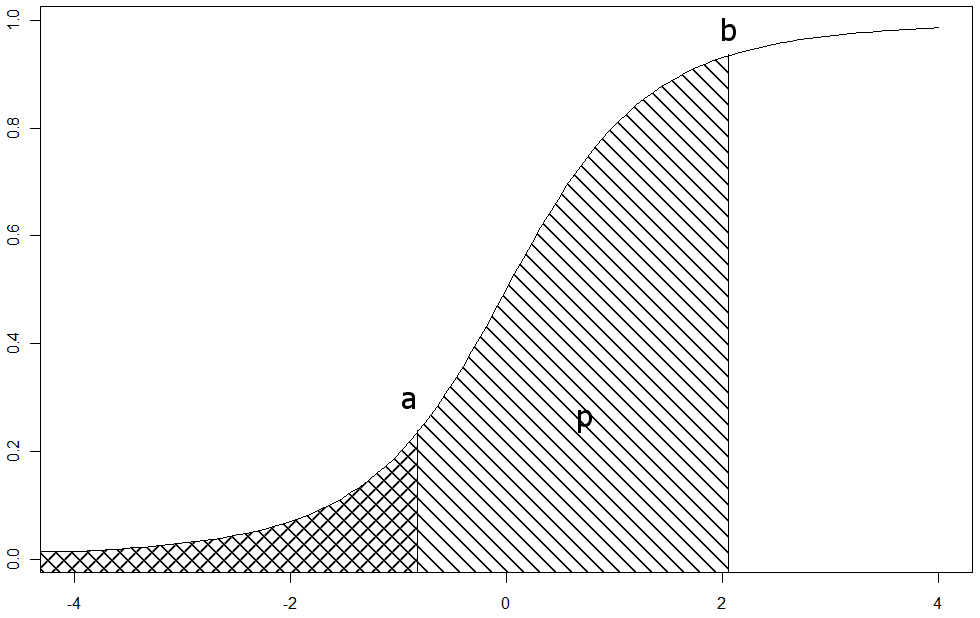
\includegraphics[scale=0.2]{fig/p}
\caption{
	\label{fig:Probability-p-that}
	Cumulative distribution function of the ratio $k/l$ between the items $k$ and $l$ (area $p$ denotes probability that $k/l$ is between $\frac{3}{4}$ and $\frac{4}{3}$.)
}
\end{figure}

After both prioritization items are tested for equality it may
be convenient to display the equality of different items in the form of a table.
Please see Table~\ref{tab:ECVexample} for an example.

\begin{table}
	\scriptsize
	\centering
\caption{Example of equality table}

\label{tab:ECVexample}
\begin{tabular}{|c|c|c|c|c|}
\hline 
prioritization items & i1 & i2 & i3 & i4\tabularnewline
\hline\hline 
i1 & equal & equal & - & equal\tabularnewline
\hline 
i2 & equal & equal & - & -\tabularnewline
\hline 
i3 & - & - & equal & -\tabularnewline
\hline 
i4 & equal & - & - & equal\tabularnewline
\hline
\end{tabular}
\end{table}

\subsection{Grouping Prioritization Items}
When equal items are determined they must be divided into groups of equal items. Division must be performed in such a way that each two items in a group are equal. The test for equality of the items described in Section~\ref{Testing-Equality-of} is not transitive. Hence, if prioritization item $A$ is equal to $B$ and $B$ is equal to $C$ then it does not automatically imply that $A$ is equal to $C$. Therefore, there may be several ways to group the equal items. The two possible division criteria that we have considered in this study are:

\begin{enumerate}
\item Maximize the number of items that have a group.
\item Maximize the number of items in each group.
\end{enumerate}

\section{\label{results}Results}
This section presents the results of this study including the systematic literature review and the application of ECV on industry and academic data collected from the primary studies.
Data extracted from primary studies and the results of the quality evaluation are available in \cite{Rinkevics2011a}.

\subsection{State of Practice in Empirical Studies that use CV or Analyze the Results of CV (RQ 1)\label{rq1}}
The study search resulted in 634 unique studies. The search in databases revealed 180 papers, while an additional 454 papers were discovered using snowball sampling.
The study selection resulted in 40 primary studies. Hence, 94\% of the studies were excluded by the selection criteria.
Snowball sampling revealed 15 (36\%) out of all primary studies.
The study selection criteria and the number of papers excluded by each criterion are shown in Tables~\ref{tab:Paper-search-and} and \ref{tab:Paper-Selection-from}.
In total 163 of 634 studies were excluded because full text was not available.

%The review process was facilitated by the reference management software Mendeley.
All results of the study selection are available online and can be obtained by contacting the authors of this paper.
For each study we specify keywords and databases that were used to find the study.
If a study has been excluded, the exclusion criteria are provided.

The number of papers revealed by each search string and database is
presented in Table~\ref{tab:Number-of-papers}. It should be noted
that several papers were found by more than one search string or in
more than one database. Table~\ref{tab:Number-of-papers} shows that
the search string `cumulative voting' was the most frequently used
in the research community to denote CV. Therefore, researchers should use 
or reference this term when discussing CV.

To perform snowball sampling we examined the references of primary studies that were found during the database search.
References were used to search for the papers in the Google and Google Scholar search engines.
Studies that were found in the search and passed the study selection criteria were added to the set of primary studies.

After the primary studies were selected, data extraction and quality evaluation was performed by two researchers.
One researcher examined all studies while the second researcher did quality evaluation and data extraction for 10\% of the studies. 
The studies were randomly selected.
Inter-rater agreement were calculated by means of Krippendorff's alpha coefficient.
Agreement for data extraction results was 0.86 and agreement for the quality evaluation was 0.73.
According to \cite{Krippendorff2004a} it is common to require agreement above 0.8 and the lowest acceptable agreement is 0.667. Therefore, we conclude that the agreement calculated for this study is sufficient.
Ratings of the study setting, correctness, research data availability, and number of prioritization items are presented in Figure~\ref{fig:qeResults}.

\begin{figure}
	\center
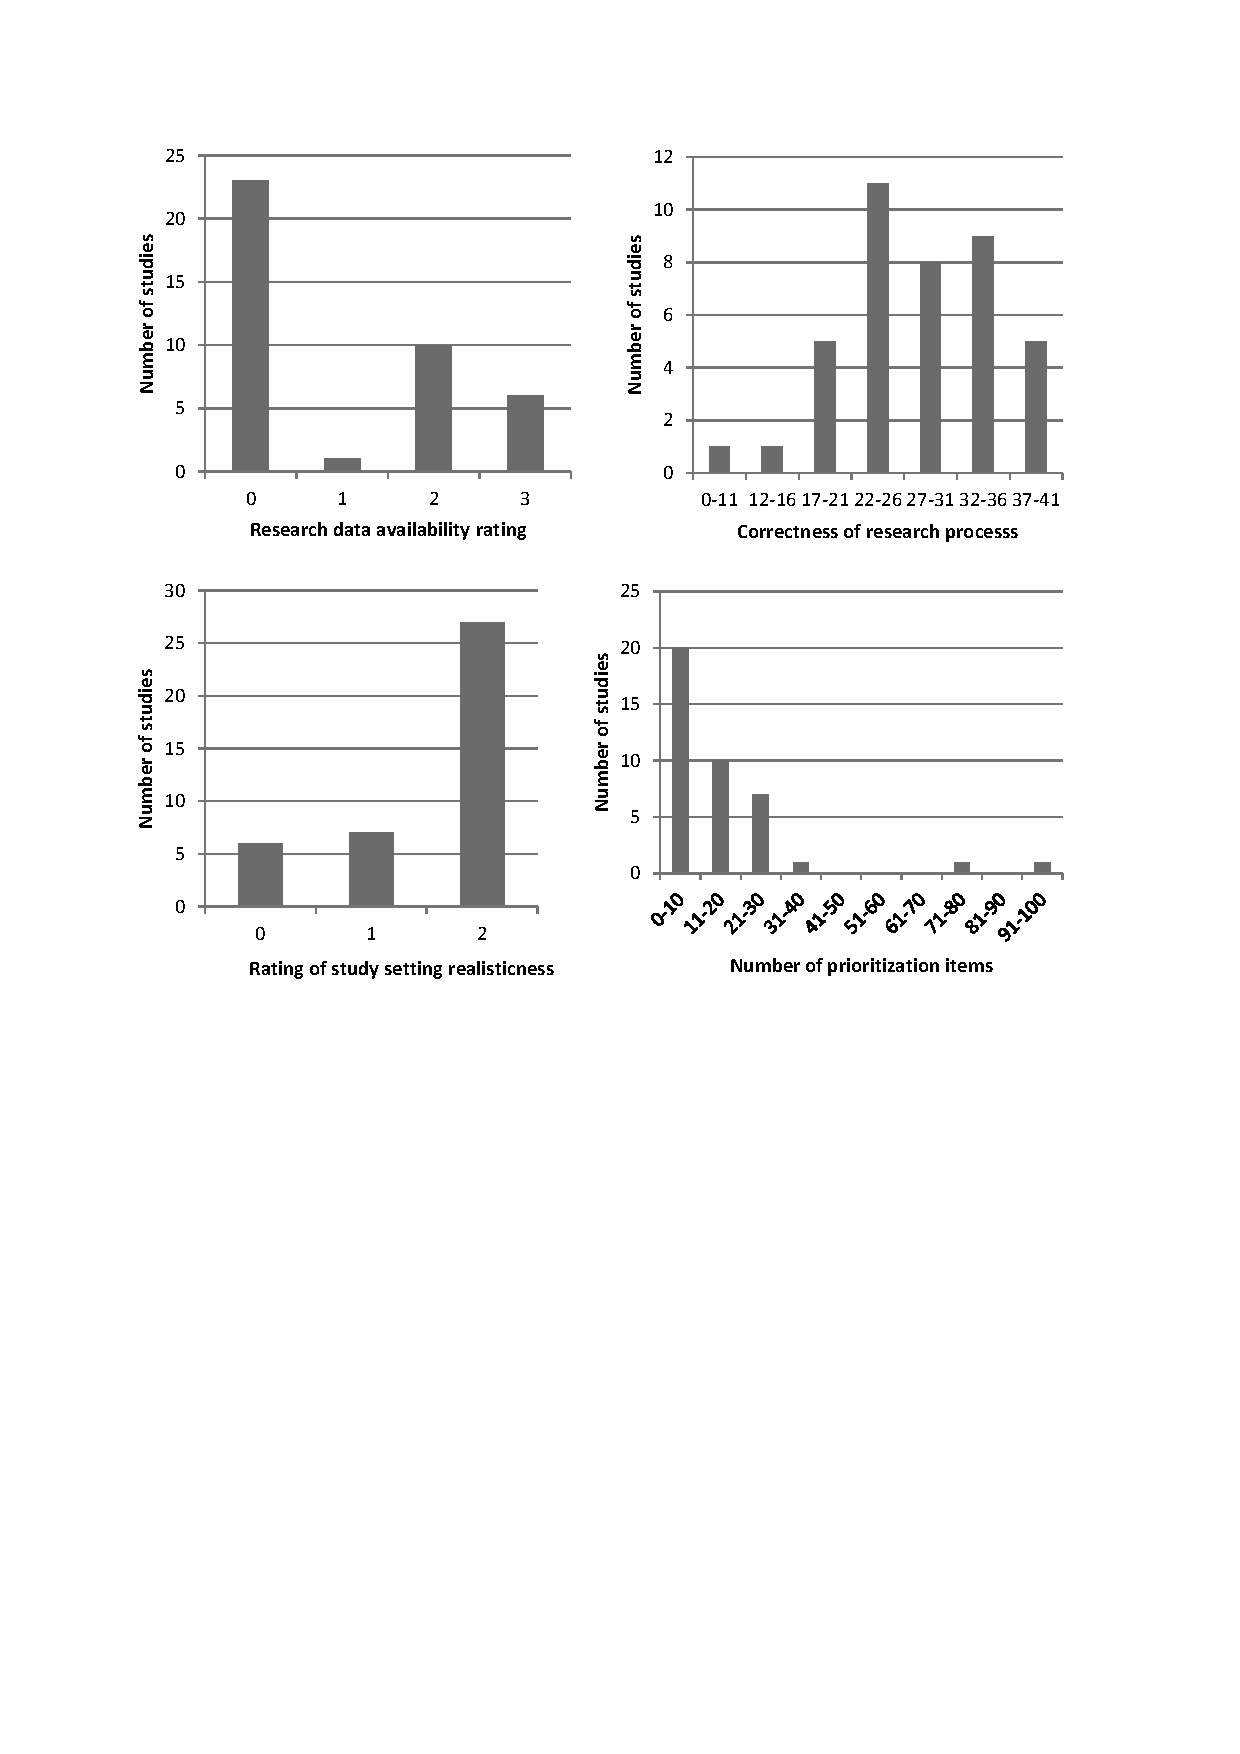
\includegraphics[bb=60bp 360bp 560bp 790bp,clip,scale=0.70]{fig/qeResults}
\caption{\label{fig:qeResults}Study quality ratings.}
\end{figure}

\begin{figure}
\center
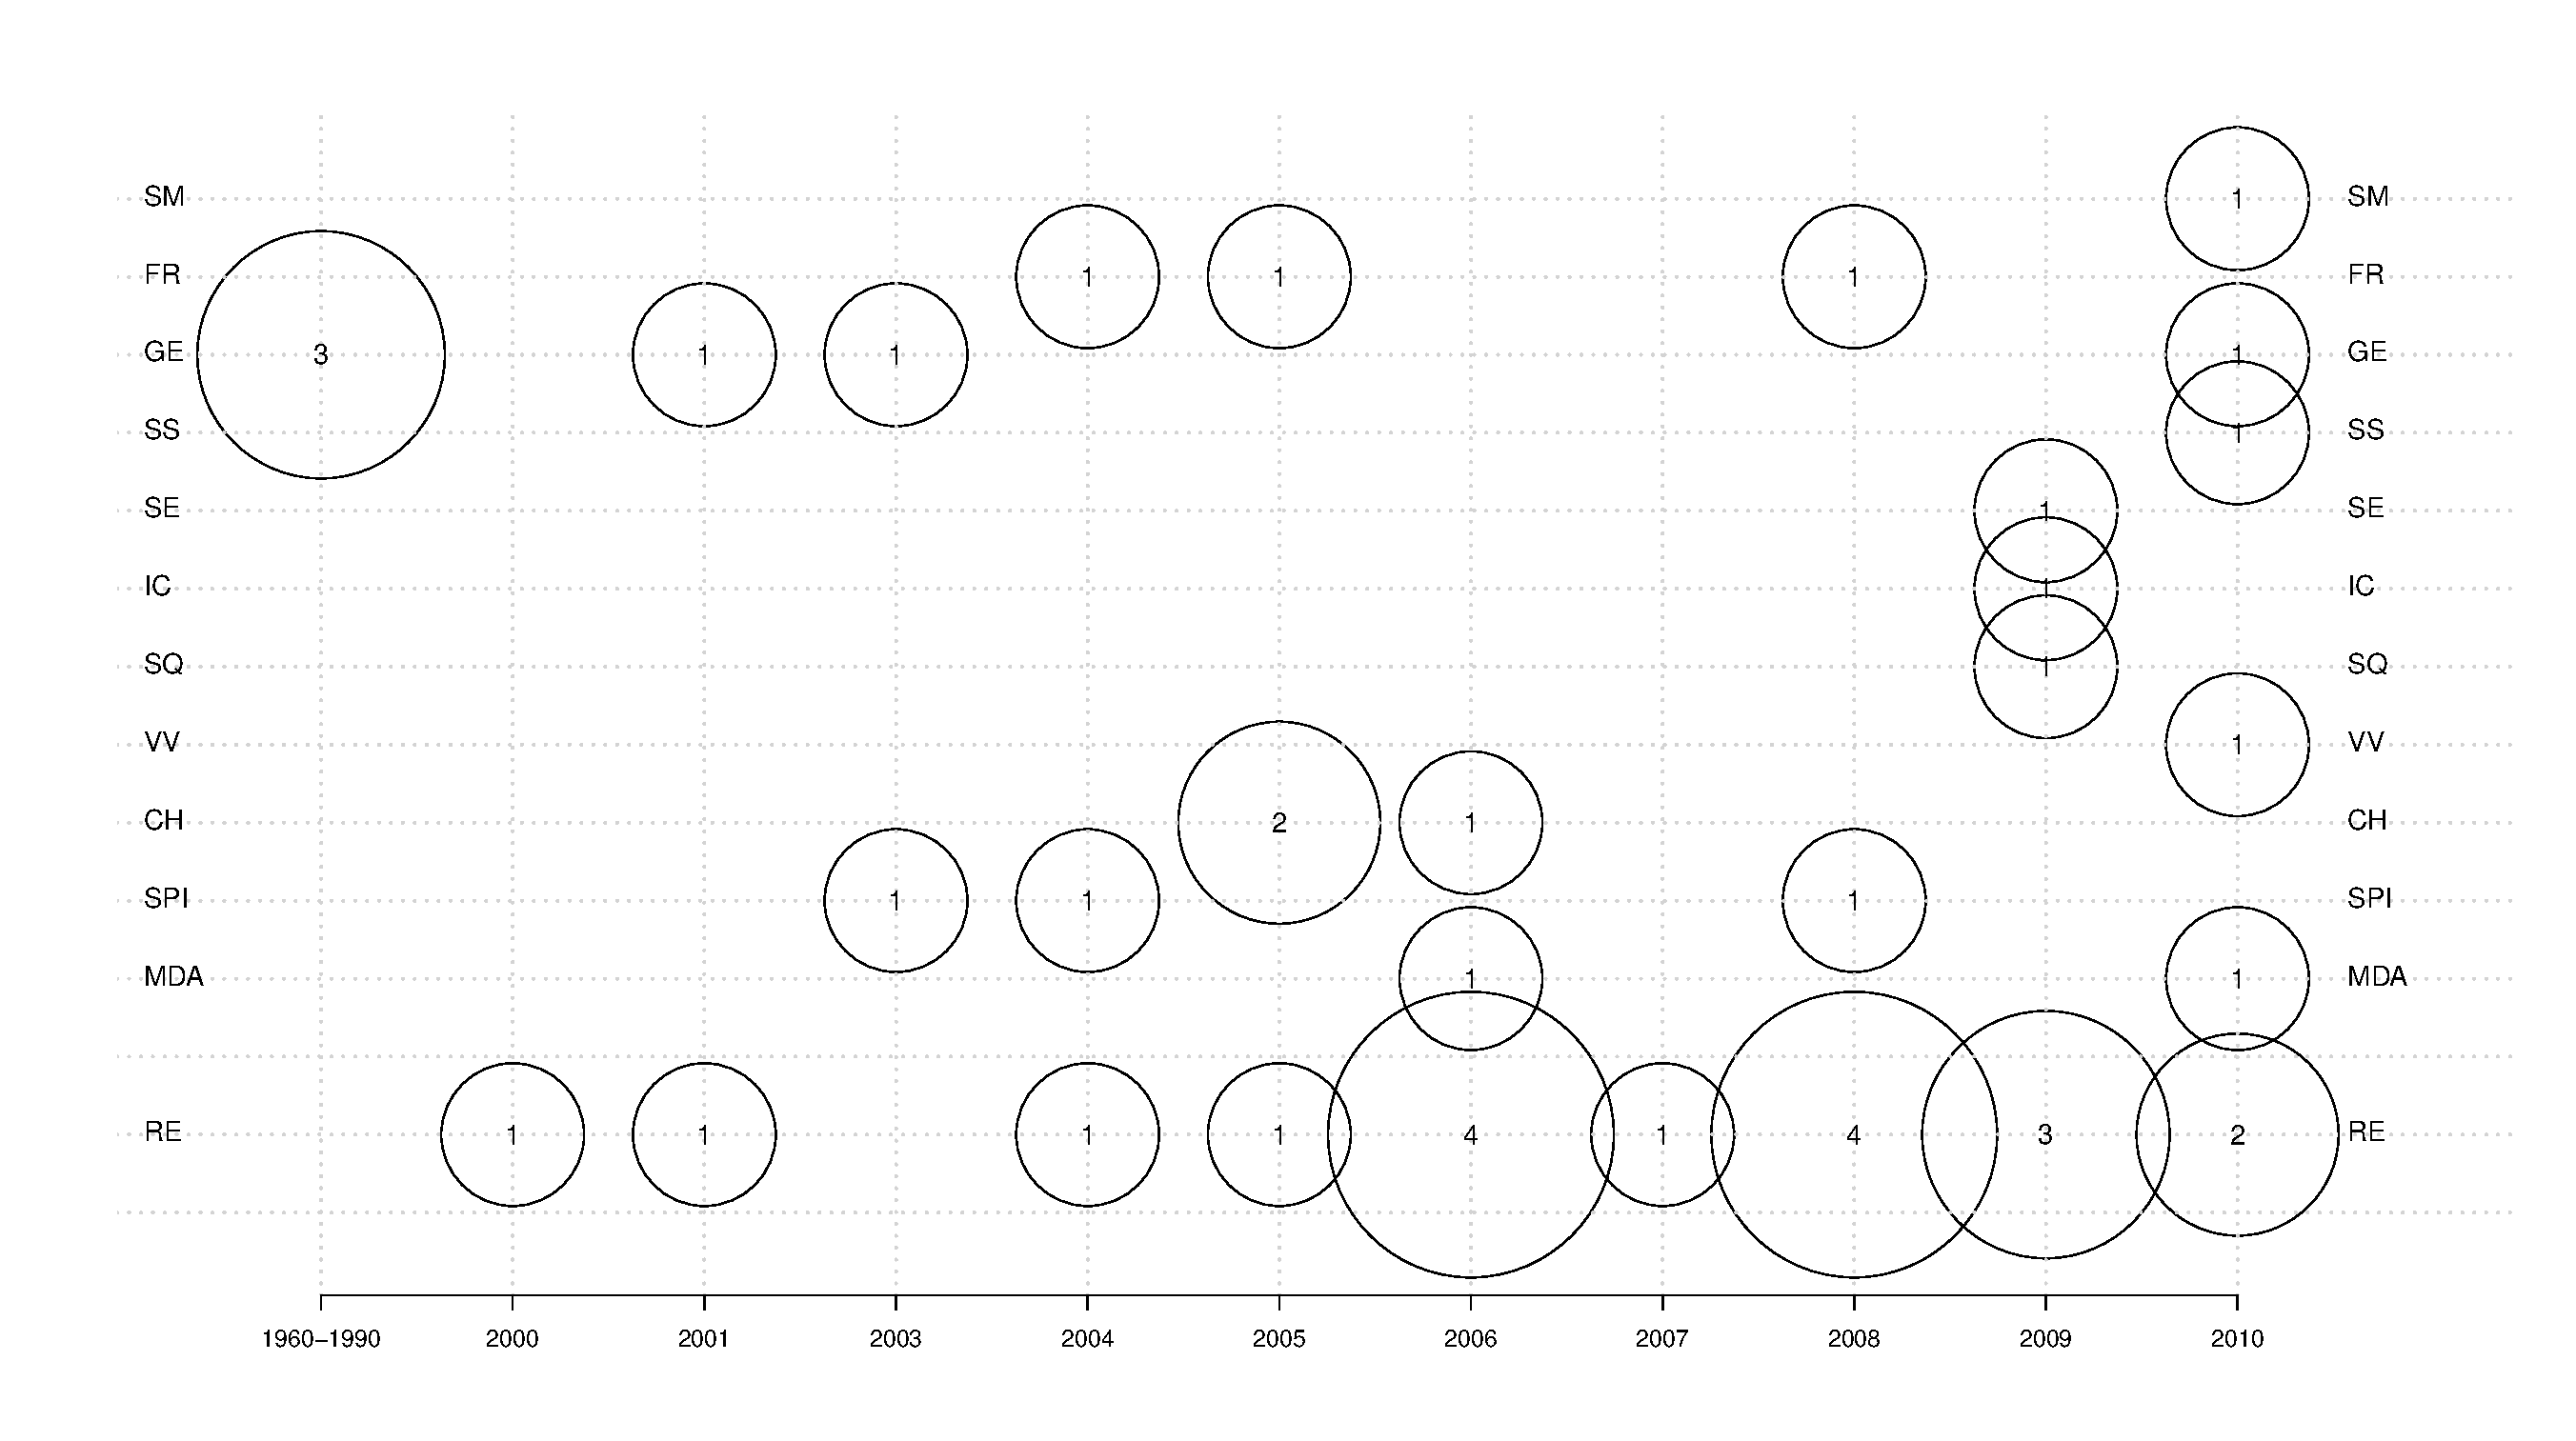
\includegraphics[bb=70bp 40bp 1180bp 670bp,clip,scale=0.28]{fig/bubble}

\begin{tabular}
{l>{\raggedright}b{0.4\columnwidth}l>{\raggedright}b{0.4\columnwidth}l} 
&\tabularnewline
\tiny
MDA - model driven software development  					& \tiny FR - forestry  \tabularnewline
\tiny CH - change impact analysis in software engineering 			& \tiny GE - government elections \tabularnewline
\tiny RE - requirements engineering and software release planning 	& \tiny SS - software security \tabularnewline
\tiny IC - intellectual capital in software company 				& \tiny SQ - software quality \tabularnewline
\tiny SPI - software process improvement 						& \tiny SM - software metrics \tabularnewline
\tiny V\&V - software verification and validation & \tiny SE - software engineering in general\tabularnewline
\end{tabular}
\caption{\label{fig:bubble}Distribution of studies over time.}

\end{figure}

Table~\ref{tab:Top-ranked} shows the studies with the highest quality according to our criteria.
These studies show a high level of rigor in a realistic setting. Moreover, authors of the studies manifest confidence by providing raw data for further use and evaluation.

Figure~\ref{fig:bubble} shows a bubble chart of the distribution of studies over research areas and time.
The figure shows that CV was, as far as we know, first applied some time ago in research of government elections.
Nowadays, though, CV has been adopted in a wide range of software engineering areas, most frequently in requirements engineering and software release planning.
Eight studies use CV in academia while the remaining 32 studies report on using CV in industry.
%\begin{flushleft}
%
%\begin{center}
\begin{table}
\center
	\scriptsize
\caption{\label{tab:Number-of-papers}Number of papers found in the databases.}

%\raggedright{}
\begin{tabular}{|>{\raggedright}b{0.3\columnwidth}|>{\raggedright}p{0.03\columnwidth}|>{\raggedright}p{0.03\columnwidth}|>{\raggedright}p{0.03\columnwidth}|>{\raggedright}p{0.03\columnwidth}|>{\raggedright}p{0.03\columnwidth}|>{\raggedright}p{0.03\columnwidth}|>{\raggedright}p{0.03\columnwidth}|>{\raggedright}p{0.03\columnwidth}|>{\raggedright}p{0.03\columnwidth}|}
\hline 
 & \multicolumn{7}{l|}{search strings} &  & \tabularnewline
\cline{2-8} 
database & \begin{sideways}
{}``100 point method''%
\end{sideways} & \begin{sideways}
{}``100 dollar method''%
\end{sideways} & \begin{sideways}
{}``100 dollar test''%
\end{sideways} & \begin{sideways}
{}``hundred point method''%
\end{sideways} & \begin{sideways}
{}``hundred dollar method''%
\end{sideways} & \begin{sideways}
{}``hundred dollar test''%
\end{sideways} & \begin{sideways}
{}``cumulative voting''%
\end{sideways} & \begin{sideways}
unique papers found%
\end{sideways} & \begin{sideways}
primary studies selected%
\end{sideways}\tabularnewline
\hline
ACM & 2 & 0 & 0 & 1 & 2 & 3 & 31 & 34 & 7\tabularnewline
\hline 
IEEE & 3 & 2 & 0 & 1 & 2 & 6 & 38 & 46 & 11\tabularnewline
\hline 
Inspec\slash Compendex & 1 & 0 & 0 & 1 & 1 & 1 & 22 & 14 & 7\tabularnewline
\hline 
ISI web of science & 0 & 0 & 0 & 0 & 1 & 1 & 15 & 16 & 6\tabularnewline
\hline 
SCOPUS & 2 & 0 & 0 & 0 & 1 & 2 & 24 & 25 & 9\tabularnewline
\hline 
Springer & 2 & 0 & 2 & 0 & 2 & 2 & 89 & 95 & 6\tabularnewline
\hline 
unique papers found & 6 & 2 & 2 & 1 & 4 & 11 & 165 & 180 & \tabularnewline
\hline 
primary studies selected & 1 & 2 & 1 & 1 & 2 & 4 & 18 &  & 25\tabularnewline
\hline
\end{tabular}%
\end{table}
%\end{center}
%\par\end{flushleft}
%
\begin{table}
	\center
	\scriptsize
\caption{\label{tab:Top-ranked}Top ranked studies.}

\begin{tabular}{|>{\raggedright}p{0.24\columnwidth}|>{\centering}p{0.15\columnwidth}|>{\centering}p{0.15\columnwidth}|
>{\centering}p{0.13\columnwidth}|>{\centering}p{0.15\columnwidth}|}
\hline 
 & Correctness of research process & Research data availability & Study setting & Number of prioritization items\tabularnewline
\hline
Barney 2009 \cite{Barney2009a} & 36 & 2 & 2 & 17\tabularnewline
\hline
Berander 2009 \cite{Berander2009a} & 41 & 2 & 0 & 29\tabularnewline
\hline
Barney 2009 \cite{Barney2009} & 40 & 2 & 2 & 5\tabularnewline
\hline
Barney 2009 \cite{Barney2009b} & 31 & 2 & 2 & 27\tabularnewline
\hline
Barney 2008 \cite{Barney2008} & 34 & 2 & 2 & 14\tabularnewline
\hline
Laukkanen 2005 \cite{Laukkanen2005a} & 22 & 3 & 2 & 30\tabularnewline
\hline
Hu 2006 \cite{Hu2006} & 34 & 2 & 1 & 14\tabularnewline
\hline
Feldt 2010 \cite{Feldt2010} & 24 & 3 & 2 & 8\tabularnewline
\hline
Regnell 2001 \cite{Regnell2001} & 21 & 3 & 2 & 91\tabularnewline
\hline
Svahnberg 2008 \cite{Svahnberg2008} & 34 & 1 & 1 & 7\tabularnewline
\hline
\end{tabular}
\end{table}
\subsection{\label{rq2}CV Result Analysis Methods Identified by RQ 1 (RQ 2)}
The papers identified in the review use various CV result analysis
methods. 
The main goals for CV result analysis are presented in Table \ref{goals_for_methods} and a summary of methods used in the primary studies can be found in Section \ref{analysisMethods}.

In order to present prioritization results many studies use charts or
tables. These charts and tables show the average priority of each prioritization item that is computed from priorities assigned by all stakeholders.
In \citep{Jonsson2005a} a table of five items with highest total priority is presented. 
\citep{Kuzniarz2010} shows tables with $min$, $max$, $\tilde{x}$, $\bar{x}$ and $\sigma$ of priorities assigned by different stakeholders to a particular prioritization item. Finally, in \citep{Rovegard2008,Kuzniarz2010} error bars are added to the chart of final priorities (denoting $\sigma$ of priorities).

In a few cases final priorities are presented in the form of ranks and CV results are degraded from ratio to ordinal scale. This is done when the interest lies only in the order of final priorities.

Several papers are interested in the difference between priorities from
different prioritization perspectives (e.g.\ current and ideal situation)
or stakeholder groups (e.g.\ software developers and management). Pearson
or Spearman correlation coefficients are commonly used to determine what 
the level of similarity is between all priorities from two perspectives.
Whereas, Wilcoxon, Kruskal-Wallis, Nemenyi-Damico-Wolfe-Dunn tests and the 
$\chi^2$ statistic are used to detect if there is a significant
difference in the value of one prioritization item from two or more perspectives. In addition, PCA is used to detect if there are distinct groups of stakeholders with common priorities \citep{Pettersson2008,Chatzipetrou2010,Wohlin2006}.

In some cases, a stakeholder may assign equal priority to several prioritization items or leave several items unrated, e.g.\ the stakeholder may not have carefully considered all prioritization items. Hence, the difference between the items may have been unnoticed.

In \citep{Berander2006a} the scalability of prioritization is measured
using two charts. The first chart shows the average percentages of items given a non-zero value. The second chart shows average percentages of divergence of values. If a stakeholder assigns equal priorities to many prioritization items the divergence of values is low. Unfortunately it is unclear from \citep{Berander2006a} how the average percentage of divergence is calculated.

In \citep{Regnell2000} distribution, disagreement, and satisfaction charts are presented.
The distribution chart shows how the final value of a prioritization
item is constructed from priorities assigned by different stakeholders.
This chart shows how much each stakeholder has contributed to the
final value of a prioritization item.
The disagreement chart shows the level of agreement between different
stakeholders on the value of a particular prioritization item.
The satisfaction chart shows stakeholder satisfaction with prioritization
results by calculating the correlation between final priorities and priorities
assigned by a stakeholder.

The use of bi-plots and ternary plots are proposed in \citep{Chatzipetrou2010}. A bi-plot shows final priorities and stakeholder viewpoints in a two dimensional plane while a ternary plot shows prioritization items inside a triangle. Ternary plots show how many low, medium or high priorities are assigned to a prioritization item. The corners of the triangle represent high, medium, and low priority, e.g.\ if a prioritization item has received mostly high priority values then it is shown closer to the high priority corner.

\begin{table}
	\scriptsize
\caption{Goals for CV result analysis.}
\label{goals_for_methods}

\begin{tabular}{|>{\raggedright}p{0.68\textwidth}|>{\raggedright}p{0.25\textwidth}|}
\hline 
Purpose of the method & Name\tabularnewline
\hline

Show the final priority of each prioritization item. Stakeholder priorities
are combined into one value. & 
Chart or table of final priorities\tabularnewline
\hline 

Difference between priorities assigned by different perspectives (status
quo, ideal situation) or different stakeholder groups (developers,
management) \citep{Chatzipetrou2010}& 
Bi-plot \tabularnewline
\hline 

detect stakeholder groups with similar priorities \citep{Chatzipetrou2010}& Bi-plot \tabularnewline
\hline 

show the relative number of issues that have received high, medium,
or low priority \citep{Chatzipetrou2010}& Ternary plot \tabularnewline
\hline 

detect stakeholder groups with common priorities \citep{Chatzipetrou2010}& PCA \tabularnewline
\hline 

how the final value of prioritization item is constructed from priorities
assigned by different stakeholder. This chart shows how much each
stakeholder has contributed to the final value of prioritization item \citep{Regnell2000}& Distribution chart  \tabularnewline
\hline 

the level of agreement between different stakeholders on value of
particular prioritization item \citep{Regnell2000} & 
Disagreement chart  \tabularnewline
\hline 

satisfaction of a stakeholder with the prioritization results by the
calculating correlation between the final priorities and priorities
assigned by a stakeholder \citep{Regnell2000}& 
Satisfaction chart\tabularnewline
\hline 

percentage of the divergence of the priorities assigned by a stakeholder \citep{Berander2006a} & 
average percentage of divergence\tabularnewline
\hline 
average percentage of items given a non-zero value \citep{Berander2006a} & \tabularnewline
\hline 

detect equal prioritization items (presented in this paper)& 
ECV \tabularnewline
\hline
\end{tabular}
\end{table}

\subsubsection{\label{codaProblems}Problems with Compositional Data Analysis in Primary Studies}

A few primary studies, as revealed by the systematic review, have problems with the analysis of compositional data.

In \citep{Wohlin2006,Pettersson2008} standard PCA is performed without applying log-ratio transformations to compositional data. According to \citep{Aitchison1983}, this is likely to be inadequate and in \citep{Filzmoser2007}, a more appropriate method for performing PCA of compositional data is shown.

The normality of compositional data is defined in \citep{PawlowskyGlahn2007}. It is stated that compositional data must first be transformed using isometric log-ratio transformation before the tests for normality can be applied. \citep{Jonsson2005a} violates this requirement by applying the Shapiro-Wilk test for normality to untransformed compositional data.

The Kruskal-Wallis test is used in \citep{Jonsson2005a} to analyze compositional data. The test is used to evaluate the difference between three organization levels. The Kruskal-Wallis test assumes that variables within each sample are independent \citep{Kruskal1952a}. However, values within compositional data vectors are not independent (as described in Section \ref{coda}). Hence, we claim the Kruskal-Wallis test to be somewhat misused in \citep{Jonsson2005a}.
\begin{table*}
\scriptsize
\caption{\label{tab:ECVresult}Identified groups of equal items.}

\begin{tabular}{|>{\centering}p{0.27\textwidth}|>{\centering}p{0.15\textwidth}|>{\centering}p{0.2\textwidth}|>{\centering}p{0.2\textwidth}|}
\hline 
Paper identifier \& Description  & Type of CV  & Pairs of equal items  & Groups of equal items\tabularnewline
\hline 
Barney 2009 \cite{Barney2009} Perceived priorities of software product investments
in an ideal situation  & comp.\ HCV & (A2, B4)

(B4, B5)

(B4, C1)

(B5, B15)

(B6, B7)

(B7, B8)

(B14, B15)

(B14, B18)

(B17, B18) & (A2, B4)

(B4, C1)

(B5, B15)

(B6, B7)

(B14, B15)

(B17, B18)\tabularnewline
\cline{2-4}
 & uncomp.\ HCV & (B4, B5)

(B4, B8)

(B5, B15)

(B6, B7)

(B7, B12)

(B14, B15)

(B14, B18)

(B16, B17)

(B12, B13) & (B4, B5)

(B5, B15)

(B6, B7)

(B14, B15)

(B16, B17)

(B12, B13)\tabularnewline
\hline 
Berander 2009 \cite{Berander2009a} Software requirements for course management system  & uncomp.\ \& comp.\ HCV  & (3:2, 3:3) & (3:2, 3:3)\tabularnewline
\hline 
Svahnberg 2008 \cite{Svahnberg2008} The view of academia researchers
on the requirements understandability criteria  & CV & (Development, Verification \& Validation)

(Development, Product Planning 1) & (Development, Product Planning 1)\tabularnewline
\hline
\end{tabular}%
\end{table*}


\subsection{Identifying Prioritization Items with Equal Priority Using ECV (RQ 3) \label{rq3}}
This section presents the results of applying ECV to the industrial and academic CV data as found through the systematic literature review. Six primary studies included the raw prioritization results in the paper itself or referenced online sources where the data was available. To collect the data from the remaining 34 papers, the authors of all papers were contacted.

First, the email addresses provided in the papers were used. If no answer was received authors were searched for using Google, Facebook and LinkedIn. Authors from 11 papers provided us with data to be used in the evaluation of ECV. However, due to confidentiality reasons we can not publish this data directly.

In short, ECV was applied to 27 CV prioritization cases from 14 studies.
In the cases of HCV, ECV was applied two times to the same data to test both compensated and uncompensated priorities. Equal items were detected in three prioritization cases. A summary of the results is presented in Table~\ref{tab:ECVresult} and below follows a summary of each relevant study.

In \cite{Svahnberg2008} a prioritization of requirement understandability criteria is presented.
One of the main findings of the paper is that two criteria - "Development" and "Verification \& Validation" -
are most important from an academic viewpoint.
ECV adds new knowledge to these results.
It shows that "Development" and "Verification \& Validation" are equally important, i.e.\ it is not true that either one of the criteria is more important.

A prioritization of software requirements for an academic course management system is presented in \cite{Berander2009a}. ECV detected that two features---Assignment Submission and Assignment Feedback---have the same priority.
If the system is developed in several releases Assignment Submission and Assignment Feedback features can be freely interchanged between the releases and, hence, in this way ECV simplifies release planning.

In \cite{Barney2009} software product investments are prioritized with HCV.
The results of ECV was different for uncompensated and compensated HCV.
When compensated HCV was used ECV detected equal items that belonged to different high level prioritization groups ($A$, $B$ and $C$) indicating that ECV provided a more fine-grained view. In the case of uncompensated HCV, on the other hand, all equal items belonged to one high level prioritization group (group $B$).


\section{Discussion and Conclusions\label{discussion}}
This section discusses the results of the systematic review and evaluation of ECV conducted as part of this study.

% state
CV has been applied in various areas, but most frequently in requirements prioritization and release planning, and quite often also as part of research methodologies.
A large part of the studies have been conducted in Sweden, at Ericsson AB.% which is currently the world's largest telecommunication equipment vendor.
One can see a slight increase in the interest in CV. During the last five years there have been more studies that use CV than between, say, 2000--2005.

% QE
Overall, studies that use CV or analyze the results of CV have a high quality in terms of correctness of research process and study realism.
However, very few studies present prioritization of more than 30 items and the availability of research data is somewhat limited. In our particular case we were able to obtain data from 43\% of the primary studies.

\subsection{Implications for Practitioners}
The results of this study provide decision support for industry practitioners.
We believe that a collection of state of the practice studies help the adoption of CV prioritization method. (The top studies are summarized in Table~\ref{tab:Top-ranked}.)
In addition, a set of CV analysis methods enables comprehensive understanding of the prioritization results. 
(The analysis methods are presented in Table~\ref{goals_for_methods}.)
One of the most common goals of CV analysis is to display the prioritization results and, thus, to show the difference between several prioritization perspectives.

Additionally, we present ECV---a novel method for CV analysis.
Prioritization often results in the assignment of similar priorities to several prioritization items.
CV results contain both `real priorities' and random errors.
Due to random errors, equal prioritization items may receive different priorities.
ECV identifies such items. It allows stakeholders to disregard the random part of the CV results.
Thus, ECV simplifies the understanding of the prioritization results.

ECV identifies prioritization items with similar priority and tests whether these items can be considered equal.
In this case, ECV can be used in software release planning.
For example, let us suppose that a set of software requirements are prioritized with regard to the implementation costs.
First of all, ECV can then detect items with equal cost.
Second, the equal items can be freely interchanged between the releases.
Finally, the decision to allocate a requirement to a particular release can be made based on another criteria, such as risk or business value.

ECV has been successfully applied on a considerable amount of CV data and, additionally, has also detected equal items in different groups of HCV hierarchies.

\subsection{Implications for Academia}
In the systematic review 36\% of papers were revealed by the snowball sampling.
That is a considerable amount.
Several studies do not mention the name of the prioritization method (i.e.\ cumulative voting or hundred dollar test).
Others are not available through selected databases because they are conference publications or theses.
It shows, in our opinion, that snowball sampling ought to be used in all systematic literature reviews.

CV results are a special type of data---compositional data.
Standard statistical analysis methods that assume the independence of the samples cannot be applied to CV results.
In \cite{Aitchison1986} methods for the analysis of compositional data have been presented.
The systematic review conducted as a part of this study revealed that 22 studies analyze CV results; yet, only one study uses compositional data analysis methods, i.e.\ \cite{Chatzipetrou2010}.
None of the studies, including \cite{Chatzipetrou2010}, present methods for detecting items with equal priority in CV results. Hence, ECV is, in this respect, a unique method.

The small use of compositional data analysis is really not surprising, since literature describing CV does not state that the results are compositional data.
Standard statistical analysis methods may produce useful results for compositional data.
However, there are cases when they are misleading or even faulty.
Section \ref{codaProblems} contains evidence of inappropriate use of statistical methods by several papers.

This study has collected a set of compositional data analysis methods for CV analysis (see Table~\ref{goals_for_methods}). 
We believe that this could help researchers to improve the analysis of CV results with appropriate methods.

Since CV is associated with compositional data, it might be tempting to choose another requirements prioritization method. However, it would not solve the problem \emph{per se}, because any ratio scale prioritization, for instance AHP, contains compositional data.

The principal implications for the academia are mainly the following:

\begin{enumerate}
\item All systematic literature reviews should include snowball sampling.
\item Researchers can improve their statistical analysis of CV results using compositional data analysis methods collected and developed by this study.
\item When CV or any other ratio scale prioritization method is taught, compositional data analysis should also be presented as part of the solution.
\end{enumerate}	

% validity
\subsection{Validity Threats}
The validity of the systematic review is mainly limited by the chosen databases, the design of the review, and human judgement in study selection and data extraction.

To mitigate the threats we use the most popular databases in the field of software engineering.
In the beginning of the systematic review a review protocol was developed, peer-reviewed, and revised.
Search strategy was validated against a set of previously known papers obtained from other researchers.

One of many terms used to name cumulative voting is `\$100 method'.
We were not able to search for this term because non of the chosen databases support search for special characters like `\$' and the search string `100 method' yields too many hits.
To increase the likelihood of discovering relevant studies snowball sampling was extensively used.

To increase the validity of study selection, all included studies and 20 randomly selected excluded studies were examined by two researchers.
There were no disagreement on the inclusion\slash exclusion of the studies.

The large number of studies identified by snowball sampling (15 out of 40 studies) may be caused by faulty design or by faulty execution of the search in the databases.
There are several reasons why the studies revealed by snowball sampling are not revealed by the search in databases. (Reason for each study is given in Table~\ref{snowPapers}.)
Based on these reasons we argue that snowball sampling does not indicate any problems with the design of the search in the databases.

Four studies were not found because they were not available through databases used in this systematic review. Out of them one is a master thesis, two are conference publications and one is a publication in the area of forestry.
Seven studies do not mention the name of the prioritization method (i.e.\ hundred dollar method or cumulative voting).
Only phrases like ``distribution of a predefined amount of fictitious money (\$100,000) over the items to be prioritized'' or ``1,000 points'' allowed us to identify that CV was indeed used. One paper used a previously unknown name for CV, i.e.\ the 100-point technique.

The quality of the data extraction and quality evaluation was validated using inter-rater agreement analysis.
In our case, 10\% of the studies were rated by two researchers and Krippendorff's alpha was calculated.
The agreement for the data extraction results was 0.86 and the agreement for the quality evaluation was 0.73 (indicating a credible level of quality).
%
%The failure to obtain raw results of several CV studies may be due to several reasons, e.g.\ the authors of the primary studies might be unwilling to communicate the data because of lack of motivation or spare time. In our case we found that we were able to minimize this threat by searching for the researchers through various channels, e.g.\ Google search, LinkedIn and Facebook.

There are two main validity threats with ECV itself.
First, ECV may not detect prioritization items with equal priority.
Second, ECV may produce a false positive result, i.e.\ there may be a real difference between items that ECV claims as being equal.

To mitigate the first threat ECV was applied on artificially created test data with and without items with similar priority.
ECV worked correctly in both cases.

To mitigate the second threat we visually inspected the results of the application of ECV on the real world data from the primary studies.
We concluded that items identified by ECV can be considered equal.

CV results used in the evaluation of ECV were tested for normality.
The tests indicated that CV results do not have multivariate normal distribution.
Therefore, the design of ECV was based on a non-parametric statistical test.

\subsection{Future Research}
There are very few studies that apply CV on prioritization sets of more than 30 items.
However, in requirements engineering, industry practitioners need to prioritize much larger numbers of software requirements.
Therefore, the state of art could benefit from the application of CV and HCV to large prioritization sets.

The proposed method, ECV, has now been evaluated on existing research data. To further evaluate the ECV, it could be applied in direct industry practice and in prioritization cases with a larger number of prioritization items.
Additionally, compositional data analysis methods, as the ones identified by this paper, should be tried with other prioritization methods that produce ratio scale results.

% new
ECV may be improved to find groups of equal items not just pairs.
Equality of a pair (or a group) of items to another item can be tested with the help of compositional  balances.

CV process can be improved with the help of compositional data analysis.
Weighting of stakeholder priorities could be done using compositional powering better than using a multiplication that will be removed in a log-ratio.

Compensation of priority values in HCV is not \emph{soubcompositionally coherent}. Sequential binary partition can be used to improve the compensation.
% new

\subsection{Conclusions}
CV prioritization results are special type of data -- compositional data.
Any analysis of CV results must take into account the compositional nature of the CV results.

This study presents a systematic literature review of the empirical use of CV.
CV has been applied in various areas, but most frequently in requirements prioritization and release planning.
The review has resulted in a collection of state of the practice studies and CV result analysis methods.
We believe that it can help the adoption of CV prioritization method.

In our case, snowball sampling was performed as a part of the review.
Since it revealed 36\% out of all primary studies, 
we believe that in future snowball sampling should be used in all systematic reviews.

Additionally, we present ECV---a novel method for CV analysis.
As suggested by our evaluation, ECV is able to detect prioritization items with equal priority (i.e.\ items that have insignificant difference in priority).
The evaluation of ECV was based on the data obtained from the authors of the primary studies.

\bibliographystyle{model1-num-names}
\bibliography{library}

%\newpage
\appendix
%\renewcommand\thesection{Appendix \Alph{section}}
\section{Primary Studies\label{primaryStudies}}

\subsection{Primary studies found during search in databases.}
%\begin{table}[hp!]
\begin{center}
	\scriptsize
%\caption{Primary studies found during search in databases}
\scalebox{0.7}{

\begin{tabular}{
|>{\raggedright}p{0.9\columnwidth}
|>{\raggedright}p{0.3\columnwidth}
|}
\hline
Title & Reference\tabularnewline
\hline\hline
Prioritizing countermeasures through the countermeasure method for software security (CM-Sec) & \citet{Baca2010}\tabularnewline \hline
The relative importance of aspects of intellectual capital for software companies & \citet{Barney2009a}\tabularnewline \hline
Software product quality: Ensuring a common goal & \citet{Barney2009b}\tabularnewline \hline
Balancing software product investments & \citet{Barney2009}\tabularnewline \hline
Hierarchical cumulative voting (HCV) prioritization of requirements in hierarchies & \citet{Berander2006a}\tabularnewline \hline
A goal question metric based approach for efficient measurement framework definition & \citet{Berander2006}\tabularnewline \hline
Evaluating two ways of calculating priorities in requirements hierarchies: An experiment on hierarchical cumulative voting & \citet{Berander2009a}\tabularnewline \hline
Election systems and voter turnout: Experiments in the United States & \citet{Bowler2001}\tabularnewline \hline
A low information theory of ballot position effect & \citet{Brockington2003}\tabularnewline \hline
Prioritization of issues and requirements by cumulative Voting: A compositional data analysis framework & \citet{Chatzipetrou2010}\tabularnewline \hline
A comparison of cumulative voting and generalized plurality voting & \citet{Cooper2010}\tabularnewline \hline
Challenges with software verification and validation activities in the space industry & \citet{Feldt2010}\tabularnewline \hline
Investigating impact of business risk on requirements selection decisions & \citet{Fogelstrom2009}\tabularnewline \hline
Choosing the right prioritization method & \citet{Hatton2008}\tabularnewline \hline
Early prioritization of goals & \citet{Hatton2007}\tabularnewline \hline
Rigorous support for flexible planning of product releases: A stakeholder-centric approach and its initial evaluation & \citet{Heikkila2010}\tabularnewline \hline
Voting methods in strategic forest planning: Experiences from Mets\"{a}hallitus & \citet{Hiltunen2008}\tabularnewline \hline
Empirical extension of a classification framework for addressing consistency in model based development & \citet{Kuzniarz2010}\tabularnewline \hline
Evaluation of the multi-criteria approval method for timber-harvesting group decision support & \citet{Laukkanen2005a} \tabularnewline \hline
A practitioner's guide to light weight software process assessment and improvement planning & \citet{Pettersson2008} \tabularnewline \hline
An empirical study on views of importance of change impact analysis issues & \citet{Rovegard2008} \tabularnewline \hline
An industrial case study on the choice between language customization mechanisms & \citet{Staron2006} \tabularnewline \hline
Perspectives on requirements understandability---For whom does the teacher's bell toll? & \citet{Svahnberg2008} \tabularnewline \hline
A study on the importance of order in requirements prioritization & \citet{Svahnberg2009} \tabularnewline \hline
A structured goal based measurement framework enabling traceability and prioritization & \citet{Touseef2010} \tabularnewline \hline

\end{tabular}
} % end scale box
%\end{table}
\end{center}
\subsection{Primary studies revealed by snowball sampling.\label{snowPapers}}
%\begin{table}
	\center
	\scriptsize
%\caption{Primary studies revealed by snowball sampling\label{snowPapers}}
\scalebox{0.7}{

\begin{tabular}{
|>{\raggedright}p{0.2\columnwidth}
|>{\raggedright}p{0.5\columnwidth}
|>{\raggedright}p{0.5\columnwidth}
|}
\hline
Reference & Title & Reason why the paper is not revealed by the search in databases  \tabularnewline
\hline\hline

\citet{Ahl2005} & An experimental comparison of five prioritization methods &
Selected databases does not contain the paper, master thesis at BTH
\tabularnewline \hline

\citet{Barney2008} & A product management challenge: Creating software product value through requirements selection & 
Prioritization method name not mentioned, phrase ``1,000 points'' used instead.
\tabularnewline \hline

\citet{Berander2004a} & Differences in views between development roles in software process improvement---A quantitative comparison &
Prioritization method name not mentioned, phrase ``100 points'' used instead.
 \tabularnewline \hline

 \citet{Berander2004} & Using students as subjects in requirements prioritization &
Unknown CV name: 100-point technique
\tabularnewline \hline

 \citet{Berander2003} & Identification of key factors in software process management: A case study &
Prioritization method name not mentioned, phrase ``100 points'' used instead.
\tabularnewline \hline

\citet{Cole1990} & Cumulative voting in a municipal election: A note on voter reactions and electoral consequences &
Study published before year 2001. %rto: did you only include studies 2001--2011? Have you said that before in the paper? I might have missed that...
%kri: hmm.. see first inclusion criteria in table 3
\tabularnewline \hline

\citet{Hu2006} & Adding value to software requirements: An empirical study in the chinese software industry & 
Prioritization method name not mentioned, phrase ``1,000 points'' used instead.
\tabularnewline \hline

\citet{Jonsson2005} & A study on prioritization of impact analysis issues: A comparison between perspectives &
Selected databases does not contain the paper.
\tabularnewline \hline

\citet{Jonsson2005a} & Understanding impact analysis: An empirical study to capture knowledge on different organizational levels &
Selected databases does not contain the paper.
\tabularnewline \hline

\citet{Kuklinski1973} & Cumulative and plurality voting: An analysis of Illinois' unique electoral system &
Study published before year 2001.
\tabularnewline \hline

\citet{Laukkanen2004} & Applying voting theory in participatory decision support for sustainable timber harvesting &
Selected databases does not contain the paper.
\tabularnewline \hline

\citet{Regnell2001} & An industrial case study on distributed prioritization in market-driven requirements engineering for packaged software &
Prioritization method name not mentioned: ``distribution of a predefined amount of fictitious money (\$100,000) over the items to be prioritized.''
\tabularnewline \hline

\citet{Regnell2000} & Visualization of agreement and satisfaction in distributed prioritization of market requirements &
Prioritization method name not mentioned: ``distribution of a predefined amount of fictitious money (\$100,000) over the items to be prioritized.''
\tabularnewline \hline

\citet{Sawyer1962} & Game theory and cumulative voting in Illinois: 1902--1954 &
Study published before year 2001.
\tabularnewline \hline

\citet{Wohlin2006} & Criteria for selecting software requirements to create product value: An industrial empirical study &
Prioritization method name not mentioned: ``The subjects had 1,000 points to spend among the 13 criteria.''
\tabularnewline \hline

\end{tabular}
}
%\end{table}

\section{CV Result Analysis Methods\label{analysisMethods}}

\begin{table}[h!]
\caption{CV result analysis methods used in papers}
\scalebox{0.6}{

\begin{tabular}{
|>{\raggedright}b{0.5\textwidth}|>{\raggedright}p{0.01\textwidth}|>{\raggedright}p{0.01\textwidth}|>{\raggedright}p{0.01\textwidth}|>{\raggedright}p{0.01\textwidth}|>{\raggedright}p{0.01\textwidth}|>{\raggedright}p{0.01\textwidth}|>{\raggedright}p{0.01\textwidth}|>{\raggedright}p{0.01\textwidth}|>{\raggedright}p{0.01\textwidth}|>{\raggedright}p{0.01\textwidth}|>{\raggedright}p{0.01\textwidth}|>{\raggedright}p{0.01\textwidth}|>{\raggedright}p{0.01\textwidth}|>{\raggedright}p{0.01\textwidth}|>{\raggedright}p{0.01\textwidth}|>{\raggedright}p{0.01\textwidth}|>{\raggedright}p{0.01\textwidth}|>{\raggedright}p{0.01\textwidth}|>{\raggedright}p{0.01\textwidth}|>{\raggedright}p{0.01\textwidth}|>{\raggedright}p{0.01\textwidth}|>{\raggedright}p{0.01\textwidth}|}
\hline
 & \multicolumn{22}{c|}{Paper}\tabularnewline
\hline
analysis method & \begin{sideways}
Svahnberg2008%
\end{sideways} & \begin{sideways}
Svahnberg2009%
\end{sideways} & 
\begin{sideways} Staron2006 \end{sideways}
 & \begin{sideways} Pettersson2008% 
\end{sideways} & \begin{sideways}
Wohlin2006%
\end{sideways} & \begin{sideways}
Laukkanen2005a%
\end{sideways} & \begin{sideways}
Hu2006%
\end{sideways} & \begin{sideways}
Jonsson2005a%
\end{sideways} & \begin{sideways}
Kuzniarz2010%
\end{sideways} & \begin{sideways}
Rovegard2008%
\end{sideways} & \begin{sideways}
Berander2006a%
\end{sideways} & \begin{sideways}
Berander2004a%
\end{sideways} & 
\begin{sideways} Berander2006 \end{sideways} 
& \begin{sideways}
Feldt2010%
\end{sideways} & \begin{sideways}
Barney2009b%
\end{sideways} & \begin{sideways}
Barney2008%
\end{sideways} & \begin{sideways}
Barney2009a%
\end{sideways} & \begin{sideways}
Barney2009%
\end{sideways} & \begin{sideways}
Jonsson2005%
\end{sideways} & \begin{sideways}
Chatzipetrou2010%
\end{sideways} & \begin{sideways}
Regnell2001%
\end{sideways} & \begin{sideways}
Regnell2000%
\end{sideways}\tabularnewline
\hline

table that shows final priorities & x &  &  & x &  &  &  &  &  &  &  &  &  &  &  & x &  &  &  &  &  & \tabularnewline
\hline
chart that shows final priorities & x &  &  & x & x & x & x &  &  &  &  &  &  &  &  & x &  &  &  &  &  & \tabularnewline
\hline
table of top 5 prioritization items &  &  &  &  &  &  &  & x &  &  &  &  &  &  &  &  &  &  &  &  &  & \tabularnewline
\hline
minimal, maximal, mean, median, and standard deviation of priorities
assigned by different stakeholders &  &  &  &  &  &  &  &  & x & x &  &  &  &  &  &  &  &  &  &  &  & \tabularnewline
\hline
bar chart of prioritization results showing mean priority and standard
deviation of priorities &  &  &  &  &  &  &  &  & x & x &  &  &  &  &  &  &  &  &  &  &  & \tabularnewline
\hline
Pearson correlation coefficient &  & x &  &  &  &  &  &  &  &  &  & x &  &  &  &  &  &  &  &  &  & \tabularnewline
\hline
Nemenyi Damico Wolfe Dunn test &  &  &  &  &  &  &  &  &  &  &  &  &  & x &  &  &  &  &  &  &  & \tabularnewline
\hline
Spearmans r &  &  &  &  &  &  &  &  &  &  &  &  &  &  & x &  & x &  &  &  &  & \tabularnewline
\hline
Kruskal Wallis test &  &  &  &  &  &  &  & x &  &  &  &  &  &  &  &  &  &  &  &  &  & \tabularnewline
\hline
Wilcoxon test &  &  &  &  &  &  & x &  &  &  &  &  &  &  &  &  &  &  &  &  &  & \tabularnewline
\hline
correlation matrix &  & x &  &  &  &  &  &  &  &  &  &  &  &  & x &  & x &  &  &  &  & \tabularnewline
\hline
chart for comparing priorities from two perspectives, priorities are
points in two dimensional plane, x and y axis represent two different
perspectives &  &  &  &  &  &  &  &  &  & x &  &  &  &  &  &  &  &  & x &  &  & \tabularnewline
\hline
difference between priorities assigned by each two stakeholders using
Chi-square statistic &  &  &  &  &  &  &  &  &  & x &  &  &  &  &  &  &  &  &  &  &  & \tabularnewline
\hline
median ranks &  & x &  &  &  &  &  &  &  &  &  &  &  &  &  &  &  &  &  &  &  & \tabularnewline
\hline
CV results converted to priority ranks &  & x &  &  &  &  &  &  &  &  &  &  & x &  &  &  &  & x &  &  &  & \tabularnewline
\hline
PCA &  &  &  & x & x &  &  &  &  &  &  &  &  &  &  &  &  &  &  & x &  & \tabularnewline
\hline
percentage of divergence of priorities assigned by a stakeholder &  &  &  &  &  &  &  &  &  &  & x &  &  &  &  &  &  &  &  &  &  & \tabularnewline
\hline
average percentage of items given non-zero value &  &  &  &  &  &  &  &  &  &  & x &  &  &  &  &  &  &  &  &  &  & \tabularnewline
\hline
distribution chart &  &  &  &  &  &  &  &  &  &  &  &  &  &  &  &  &  &  &  &  & x & x\tabularnewline
\hline
disagreement chart &  &  &  & x &  &  &  &  &  &  &  &  &  &  &  &  &  &  &  &  & x & x\tabularnewline
\hline
satisfaction chart &  &  &  & x &  &  &  &  &  &  &  &  &  &  &  &  &  &  &  &  & x & x\tabularnewline
\hline
biplot &  &  &  &  &  &  &  &  &  &  &  &  &  &  &  &  &  &  &  & x &  & \tabularnewline
\hline
ternary plot &  &  &  &  &  &  &  &  &  &  &  &  &  &  &  &  &  &  &  & x &  & \tabularnewline
\hline

\end{tabular}
} % end the scale box
\end{table}


\section{\label{app:QE}Quality Evaluation Checklist}

%\begin{table}[hp!]
	\center
	\scriptsize
%\caption{Quality evaluation checklist}
\scalebox{0.5}{

\begin{tabular}{|>{\raggedright}p{0.04\textwidth}|>{\raggedright}p{0.3\textwidth}|>{\raggedright}p{1.3\textwidth}|>{\raggedright}p{0.09\textwidth}|}
\hline 
 & Item & Question or Description of the Item & Rating\tabularnewline
\hline 
1. & Background, introduction & Introduce research area  & \tabularnewline
\hline 
2. & Problem statement, purpose & What is the problem \cite{Jedlitschka2005}?
Where does it occur \cite{Jedlitschka2005}?

Who has observed it \cite{Jedlitschka2005}?
Why is it important to be solved \cite{Jedlitschka2005}? & \tabularnewline
\hline 
3. & Context, independent variables (aka. environment, setting) & Study location, time constraints, application domain, organization,
tools, market, process (e.g. software development methodology), size
of project, product that is being developed & \tabularnewline
\hline 
4. & Related work & Other existing work, alternative technologies, solutions, and studies & \tabularnewline
\hline 
5. & Goals and Hypotheses & Null hypothesis and one or more alternative hypotheses for each goal & \tabularnewline
\hline 
6. & Research questions &  & \tabularnewline
\hline 
\multicolumn{1}{|l|}{7.} & Design, Research methods &  & \tabularnewline
\cline{1-3}
7.1. & Design & Description of each step of the study & \tabularnewline
\cline{1-3}
7.2. & Control group & If there is a control group, are participants similar to the treatment
group participants in terms of variables that may affect study outcomes\cite{Kitchenham2007}? & \tabularnewline
\cline{1-3}
7.3. & Randomization & Random selection of participants and objects

Random assignment of treatment and objects to participants

Random order of treatments in case of paired design. If each participant
is assigned two treatments A and B, then part of participants perform
A first and the other part start with B & \tabularnewline
\cline{1-3}
7.4. & Blocking & Group participants of the study into homogeneous groups called blocks
(e.g.\ students in one course, database developers in one company)
and implement the study design within each block independently. The
idea is that variability of independent variables (e.g.\ experience
and knowledge of subjects) is smaller within a group. That helps measuring
changes in dependent variables \cite{Kitchenham2004}. & \tabularnewline
\cline{1-3}
7.5. & Balancing & Equal number of subjects should be assigned to each treatment \cite{Kitchenham2004}. & \tabularnewline
\cline{1-3}
7.6. & Blinding & Automated assignment of treatments to subjects \cite{Kitchenham2004}

Automated distribution of study materials to subjects \cite{Kitchenham2004}

Persons who grade the task results should not know which treatment
was used \cite{Kitchenham2004}

Analyst should not know which treatment group is which \cite{Kitchenham2004}

Automated data collection from subjects \cite{Kitchenham2004} & \tabularnewline
\hline 
\multicolumn{1}{|l|}{8.} & Subjects (participants) &  & \tabularnewline
\cline{1-3}
8.1. & Population &  & \tabularnewline
\cline{1-3}
8.2. & Sampling & How sampling is performed?

What subjects are included and excluded? \cite{Kitchenham2007}

What is the type of the sampling (e.g.\ convenience, random)?

Is the sample(selected participants) representative of the population? & \tabularnewline
\cline{1-3}
8.3. & {}``Drop outs'' and response rate & Are reasons given for refusal to participate\cite{Kitchenham2007}? & \tabularnewline
\cline{1-3}
8.4. & Subject motivation & E.g.\ material benefits, course credits for students, etc. & \tabularnewline
\hline 
9. & Objects & E.g.\ documents and other artifacts & \tabularnewline
\hline 
10. & Measures, Data collection procedures & Who, when, and how to measure \cite{Kitchenham2007}?

How is the measurement supported? Is it automated \cite{Kitchenham2007}?

Are the measures used in the study the most relevant ones for answering
the research questions \cite{Kitchenham2007}? & \tabularnewline
\hline 
\multicolumn{1}{|l|}{11.} & Analysis procedure &  & \tabularnewline
\cline{1-3}
11.1. & Data description & Do the numbers add up across different tables and subgroups \cite{Kitchenham2007}? & \tabularnewline
\cline{1-3}
11.2. & Data types (continuous, ordinal, categorical) &  & \tabularnewline
\cline{1-3} 
11.3. & Scoring systems &  & \tabularnewline
\cline{1-3}
11.4. & Data set reduction, outliers &  & \tabularnewline
\cline{1-3}
11.5. & Statistical methods & Are the assumptions of statistical methods met?

What statistical programs are used? & \tabularnewline
\cline{1-3}
11.6. & Statistical significance & If statistical tests are used to determine differences, is the actual $p$-value given \cite{Kitchenham2007}?

If the study is concerned with differences among groups, are confidence
limits given describing the magnitude of any observed differences
\cite{Kitchenham2007}? & \tabularnewline
\hline 
12. & Validity threats & Threats, implications of the threats, and threat mitigation & \tabularnewline
\cline{1-3}
12.1. & Side-effects during study execution & Deviations from the plan, solutions for the deviations & \tabularnewline
\hline 
13. & Most important findings  & Are all study questions answered \cite{Kitchenham2007}?

Are negative findings presented \cite{Kitchenham2007}? & \tabularnewline
\hline 
14. & Industry impact, inference, generalization & What implications does the report have for practice \cite{Kitchenham2007}?

How and where the results can be used?

Limitations under which findings are relevant \cite{Jedlitschka2005}? & \tabularnewline
\hline 
15. & Future work &  & \tabularnewline
\hline

\end{tabular}
} % end scale box
%\end{table}

%% The Appendices part is started with the command \appendix;
%% appendix sections are then done as normal sections
%% \appendix

%% \section{}
%% \label{}

%% References
%%
%% Following citation commands can be used in the body text:
%% Usage of \cite is as follows:
%%   \cite{key}          ==>>  [#]
%%   \cite[chap. 2]{key} ==>>  [#, chap. 2]
%%   \citet{key}         ==>>  Author [#]

%% References with bibTeX database:

\bibliographystyle{model1a-num-names}
\bibliography{library}

%% Authors are advised to submit their bibtex database files. They are
%% requested to list a bibtex style file in the manuscript if they do
%% not want to use model1a-num-names.bst.

%% References without bibTeX database:

% \begin{thebibliography}{00}

%% \bibitem must have the following form:
%%   \bibitem{key}...
%%

% \bibitem{}

% \end{thebibliography}


\end{document}

%%
%% End of file `elsarticle-template-1a-num.tex'.
